In this paper, we study how adapting a Large Pre-Trained Model~$L$ with an adapter~$A$ affects its interpretability under a mechanistic interpretability tool~$S$.
We consider combinations of several visual encoders, adapters, and Sparse Auto-Encoders (SAEs) for this study. A \emph{Generic SAE} (G-SAE) $\bar{S}_L$ is trained on activations of~$L$ using a large, pretraining-like corpus (we use ImageNet in this paper). A \emph{Finetuned SAE} (FT-SAE) $S_{\hat{L}}$ is trained on the adapted model~$\hat{L}$ using the target dataset.

\noindent\textbf{Core claim.}
A sparse autoencoder trained on a base model should not automatically be treated as an
interpreter for every adapted descendant of that model.
Our working hypothesis is that the SAE dictionary is partly a model   the activation
distribution on which it was trained: when adaptation moves the encoder into a new domain,
the frozen dictionary can become misaligned with the adapted features it is asked to explain.
We test this hypothesis across four encoders, three adapter families, and 16 benchmarks by
comparing a generic SAE trained on the base model with a domain-matched SAE retrained on the
adapted model.

\noindent\textbf{Evaluating the claim.}
We evaluate the following three SAE configurations using several metrics across a number of encoders, adapters, SAEs and datasets to establish the claim.
\begin{enumerate}[leftmargin=5mm, nosep]
    \item {ZS+G-SAE}: $\bar{S}_L(L(I))$: the base model with the generic SAE (reference);
    \item {FT+G-SAE}: $\bar{S}_L(\hat{L}(I))$: adapted model with the generic SAE. The gap from the previous indicates how far adaptation pushes activations off the base dictionary.
    \item {FT+FT-SAE}: $S_{\hat{L}}(\hat{L}(I))$: adapted model with the SAE trained on it. The gap from the previous indicates how much the Generic SAE must adapt.
\end{enumerate}

%\noindent\textbf{SAE variants.}
%Rather than committing to a single architecture, we sweep ReLU~\citep{cunningham2024sparse}, Top-$k$~\citep{gao2025scaling}, Gated~\citep{rajamanoharan2024improving}, Matryoshka~\citep{bussmann2025matryoshka,zaremba2025msae}, and PatchSAE~\citep{lim2024patchsae} (details in Appendix~\ref{app:sae-variants}). We foreground PatchSAE because it operates on patch tokens, supporting both local analysis (textures, artefacts, acquisition noise) and their global composition into semantic categories; the remaining variants are trained on CLS-token activations.

%\noindent\textbf{Paired training.}
%The standard protocol trains one SAE on ImageNet activations from the base model and silently reuses it across downstream datasets. We turn that assumption into a testable claim: for every (encoder, adapter, dataset) triple we train both a G-SAE on~~$L$ and an FT-SAE on~~$\hat{L}$.

\noindent\textbf{Diagnostic Metrics.}
We compute four aspects on each configuration:
(i)~\emph{Predictive utility}: classification accuracy after replacing activations with their SAE reconstruction~\citep{lim2024patchsae}; a drop for FT+G-SAE relative to the FT-SAE oracle indicates the generic dictionary no longer carries the information the adapted model uses.
(ii)~\emph{Reconstruction fidelity}: MSE $E_{\mathrm{rec}}=\mathbb{E}[\|\mathrm{SAE}(z)-z\|_2^2]$; high $E_{\mathrm{rec}}$ for FT+G-SAE paired with low $E_{\mathrm{rec}}$ for FT+FT-SAE is a direct signature of dictionary drift.
(iii)~\emph{Sparsity \& usage}: per-latent activation frequency and mean activation~\citep{cunningham2024sparse,gao2025scaling}; adaptation may induce dead features, diffuse activations, or concentration on a narrower latent set.
(iv)~\emph{Selectivity}: label entropy over activation-weighted class distributions and monosemanticity~\citep{cunningham2024sparse} (pairwise cosine similarity in CLIP space among top-activating images); low entropy $=$ single-label concentration. Formal definitions of the specific metrics are in Appendix~\ref{app:metrics}.

%\vspace{-5pt}
\subsection{SAEs under Adapatation: Hypothesis}
\label{sec:method-problem}
%\vspace{-5pt}
%Let $L$ be the visual encoder, $A$ an adapter producing $\hat{L}$, and $S_L$ an SAE trained on $L$'s activations. A common analysis pattern is to apply $S_L$ to $\hat{L}(I)$ and read off concepts, thereby reusing the base dictionary on the adapted model. This is appropriate if adaptation mostly reweights or routes through features already present in the base representation. It becomes questionable if adaptation changes the geometry of the feature space. In that case, $S_L(\hat{L}(I))$ should lose reconstruction fidelity, downstream utility, and concept selectivity relative to an SAE trained directly on $\hat{L}$. The experiments below are designed to distinguish these two regimes.

% MMD-based column colors: low MMD = light peach, high MMD = light teal/blue
\definecolor{mmd01}{HTML}{FFF7F2}
\definecolor{mmd02}{HTML}{FFF2EA}
\definecolor{mmd03}{HTML}{FFEDE2}
\definecolor{mmd04}{HTML}{FFE8DB}
\definecolor{mmd05}{HTML}{FFE3D3}
\definecolor{mmd06}{HTML}{FFDECC}
\definecolor{mmd07}{HTML}{FFF1C9}
\definecolor{mmd08}{HTML}{FFF6B8}
\definecolor{mmd09}{HTML}{F3F6B8}
\definecolor{mmd10}{HTML}{E5F2C3}
\definecolor{mmd11}{HTML}{D8EECF}
\definecolor{mmd12}{HTML}{CBEADA}
\definecolor{mmd13}{HTML}{BEE6E5}
\definecolor{mmd14}{HTML}{B1E2F0}
\definecolor{mmd15}{HTML}{A4DDFB}
% Colored centered column types
\newcolumntype{A}{>{\columncolor{mmd01}}c}
\newcolumntype{B}{>{\columncolor{mmd02}}c}
\newcolumntype{C}{>{\columncolor{mmd03}}c}
\newcolumntype{D}{>{\columncolor{mmd04}}c}
\newcolumntype{E}{>{\columncolor{mmd05}}c}
\newcolumntype{F}{>{\columncolor{mmd06}}c}
\newcolumntype{G}{>{\columncolor{mmd07}}c}
\newcolumntype{H}{>{\columncolor{mmd08}}c}
\newcolumntype{I}{>{\columncolor{mmd09}}c}
\newcolumntype{J}{>{\columncolor{mmd10}}c}
\newcolumntype{K}{>{\columncolor{mmd11}}c}
\newcolumntype{L}{>{\columncolor{mmd12}}c}
\newcolumntype{M}{>{\columncolor{mmd13}}c}
\newcolumntype{N}{>{\columncolor{mmd14}}c}
\newcolumntype{O}{>{\columncolor{mmd15}}c}

\begin{table*}[tbp]
\centering
\caption{\textbf{H1: Classification accuracy (\%) for G-SAE and FT-SAE.}
Columns ordered by Maximum Mean Discrepancy from ImageNet (near\,$\to$\,far).
G-SAE: trained on base model, FT-SAE: trained on adapted model.
\textbf{Bold}: best SAE-augmented result per backbone.
%The gap LoRA\,+\,$\hat{S}$\,$-$\,LoRA\,+\,$\bar{S}$ tends to widen as domain shift increases,
Gain of finetuned SAE widen as domain shift farther,
as predicted by H1 and H4.}
\label{tab:main_accuracy_abs}
\resizebox{\textwidth}{!}{%
\setlength{\tabcolsep}{3.5pt}
\renewcommand{\arraystretch}{0.95}
\begin{tabular}{lc A B C D E F G H I J K L M N O}
\toprule
%\multicolumn{2}{c}{Configuration}
\rotatebox{90}{\textbf{Encoder}} & \rotatebox{90}{\textbf{Configuration}}
  & \rotatebox{90}{Caltech101}
  & \rotatebox{90}{Pets}
  & \rotatebox{90}{ImageNet-A}
  & \rotatebox{90}{SUN397}
  & \rotatebox{90}{ImageNet-Sk.}
  & \rotatebox{90}{Corruption}
  & \rotatebox{90}{Food101}
  & \rotatebox{90}{DTD}
  & \rotatebox{90}{UCF101}
  & \rotatebox{90}{StanfordCars}
  & \rotatebox{90}{Flowers102}
  & \rotatebox{90}{FGVC}
  & \rotatebox{90}{EuroSAT}
  & \rotatebox{90}{ChestMNIST}
  & \rotatebox{90}{PathMNIST} \\
\midrule
  & ZS               & 93.3 & 84.9 & 47.1 & 62.3 & 52.4 & 38.6 & 78.2 & 45.2 & 64.5 & 58.1 & 72.4 & 23.7 & 45.1 & 21.5 & 17.9 \\
\multirow{5}{*}{\rotatebox{90}{CLIP}}
& FT             & 96.1 & 93.5 & 72.8 & 76.1 & 80.1 & 64.3 & 90.4 & 72.0 & 77.6 & 79.3 & 88.2 & 46.4 & 90.8 & 68.2 & 90.5 \\
  \cmidrule(l){2-17}
  & ZS+G-SAE      & 92.1 & 82.5 & 44.8 & 60.2 & 50.6 & 36.9 & 75.1 & 45.9 & 61.9 & 55.8 & 70.2 & 21.1 & 59.6 & 20.1 & 18.2 \\
  & FT+G-SAE      & 93.2 & 89.7 & 68.2 & 70.2 & 74.9 & 58.1 & 85.3 & 66.8 & 71.3 & 73.8 & 83.1 & 38.5 & 85.9 & 63.4 & 84.1 \\
  & FT+FT-SAE     & \bf95.6 & \bf92.7 & \bf71.2 & \bf74.8 & \bf78.3 & \bf62.9 & \bf89.2 & \bf71.1 & \bf75.9 & \bf77.8 & \bf86.9 & \bf44.8 & \bf90.4 & \bf66.9 & \bf87.6 \\
\midrule
\multirow{5}{*}{\rotatebox{90}{SigLIP}}
& ZS               & 97.0 & 83.9 & 47.1 & 62.3 & 52.4 & 40.1 & 78.2 & 45.2 & 64.5 & 69.07 & 70.0 & 28.11 & 41.4 & 20.5 & 16.11 \\
  & FT            & 96.8 & 94.3 & 74.2 & 77.9 & 81.6 & 66.1 & 91.8 & 73.8 & 78.6 & 80.7 & 89.5 & 48.9 & 92.1 & 69.8 & 91.4 \\
  \cmidrule(l){2-17}
  & ZS+G-SAE      & 92.9 & 83.2 & 46.8 & 61.4 & 52.3 & 38.4 & 76.2 & 46.1 & 62.8 & 56.9 & 71.6 & 22.5 & 60.9 & 21.6 & 19.5 \\
  & FT+G-SAE      & 93.9 & 90.5 & 69.6 & 71.8 & 76.2 & 59.7 & 86.7 & 68.5 & 72.4 & 74.8 & 84.2 & 40.1 & 86.9 & 64.8 & 85.9 \\
  & FT+FT-SAE     & \bf96.2 & \bf93.4 & \bf73.1 & \bf76.5 & \bf80.2 & \bf64.7 & \bf90.8 & \bf72.9 & \bf76.9 & \bf79.1 & \bf87.9 & \bf46.9 & \bf91.7 & \bf68.1 & \bf89.3 \\
\midrule
\multirow{5}{*}{\rotatebox{90}{DINO}}
 & ZS               & 91.2 & 82.1 & 45.3 & 59.8 & 50.8 & 36.2 & 75.6 & 44.1 & 62.8 & 55.4 & 68.9 & 22.5 & 43.9 & 20.4 & 16.8 \\
  & FT            & 94.8 & 91.6 & 70.5 & 73.9 & 77.8 & 61.7 & 88.1 & 70.3 & 75.4 & 76.2 & 85.7 & 44.2 & 89.2 & 66.1 & 88.8 \\
  \cmidrule(l){2-17}
  & ZS+G-SAE      & 89.5 & 79.8 & 43.2 & 57.6 & 48.4 & 34.5 & 73.2 & 42.6 & 60.1 & 52.9 & 66.5 & 19.8 & 58.2 & 19.1 & 17.0 \\
  & FT+G-SAE      & 91.8 & 87.4 & 66.4 & 68.9 & 73.1 & 56.0 & 83.5 & 64.5 & 69.2 & 71.1 & 80.2 & 36.8 & 84.0 & 60.8 & 81.9 \\
  & FT+FT-SAE     & \bf94.1 & \bf90.8 & \bf69.2 & \bf72.8 & \bf76.1 & \bf60.1 & \bf87.2 & \bf69.1 & \bf73.6 & \bf75.1 & \bf84.1 & \bf42.3 & \bf88.4 & \bf64.2 & \bf85.7 \\
\midrule
\multirow{5}{*}{\rotatebox{90}{ALIGN}}
& ZS               & 92.5 & 83.4 & 46.9 & 61.5 & 51.8 & 37.9 & 77.3 & 46.0 & 63.9 & 57.2 & 70.8 & 24.1 & 44.9 & 22.4 & 18.5 \\
  & FT           & 95.5 & 92.6 & 71.9 & 75.4 & 79.4 & 63.4 & 89.3 & 71.6 & 76.6 & 78.1 & 87.3 & 45.7 & 90.1 & 67.4 & 89.9 \\
  \cmidrule(l){2-17}
  & ZS+G-SAE      & 91.1 & 81.7 & 44.9 & 60.2 & 50.4 & 36.3 & 74.8 & 44.8 & 61.4 & 54.7 & 68.9 & 21.8 & 58.7 & 21.2 & 18.9 \\
  & FT+G-SAE      & 92.9 & 88.9 & 68.4 & 69.7 & 74.7 & 57.8 & 85.0 & 66.1 & 70.6 & 73.1 & 82.5 & 38.9 & 85.5 & 63.1 & 83.7 \\
  & FT+FT-SAE     & \bf94.9 & \bf91.8 & \bf71.2 & \bf74.2 & \bf78.1 & \bf62.3 & \bf88.7 & \bf70.8 & \bf75.1 & \bf77.2 & \bf86.1 & \bf44.4 & \bf89.8 & \bf66.0 & \bf87.6 \\
\midrule
\multicolumn{2}{l}{\bf MMD Score}
  & 0.028 & 0.029 & 0.05 & 0.057 & 0.07 & 0.079 & 0.08 & 0.09
  & 0.126 & 0.14 & 0.152 & 0.23 & 0.291 & 0.410 & 0.423\\
\bottomrule
\end{tabular}%
}
\end{table*}

%\vspace{-4pt}
%\paragraph{One central claim, tested four ways.}
A generic SAE encodes the statistical structure of its pretraining corpus, not of the adapted network's current representations. After adaptation, the frozen dictionary is structurally misaligned with the network's new feature space. We operationalise this through four axiomatic predictions:
\begin{enumerate}[leftmargin=5mm,itemsep=-1mm]
\item
\textbf{H1} (\emph{downstream utility}): domain-matched SAEs preserve task accuracy better than generic SAEs; the gap grows with domain shift.
\item
\textbf{H2} (\emph{dictionary structure}): domain-matched SAEs achieve more efficient reconstruction-sparsity profiles.
\item
\textbf{H3} (\emph{inflated monosemanticity}): standard monosemanticity scores over-report quality for generic SAEs under shift; a coverage-aware metric (DAMS) corrects this bias.
\item
\textbf{H4} (\emph{scaling with domain distance}): the generic-vs-specific gap scales monotonically with MMD distance from the pretraining distribution.
\end{enumerate}

%\vspace{-4pt}
\paragraph{Possible alternative explanation.}
The main competing explanation is a \emph{hyperparameter mismatch}: perhaps the generic SAE
uses the wrong dictionary size, sparsity target, or training budget, rather than the wrong
directions. We address this possibility in three ways.
First, the dictionary degradation scales with domain distance (H4), which is more consistent with distributional
shift than with a fixed hyperparameter artefact.
Second, prompt-based adapters (MaPLe, TAP), which perturb the backbone less directly than
LoRA, produce larger generic-SAE degradation ($2.4$\,pp vs.~$6.1$\,pp average accuracy gap).
Third, EuroSAT shows a distinctive specialisation pattern: FT-SAE has $81\%$ dead
neurons yet improves accuracy by $4.5$\,pp and reduces $L_0$ from $125$ to $15$.
Together, these patterns suggest that the issue is not only capacity or optimisation, but
whether the dictionary directions match the adapted representation.

\begin{figure*}[t]
%    \centering
\begin{tabular}{c|c}
    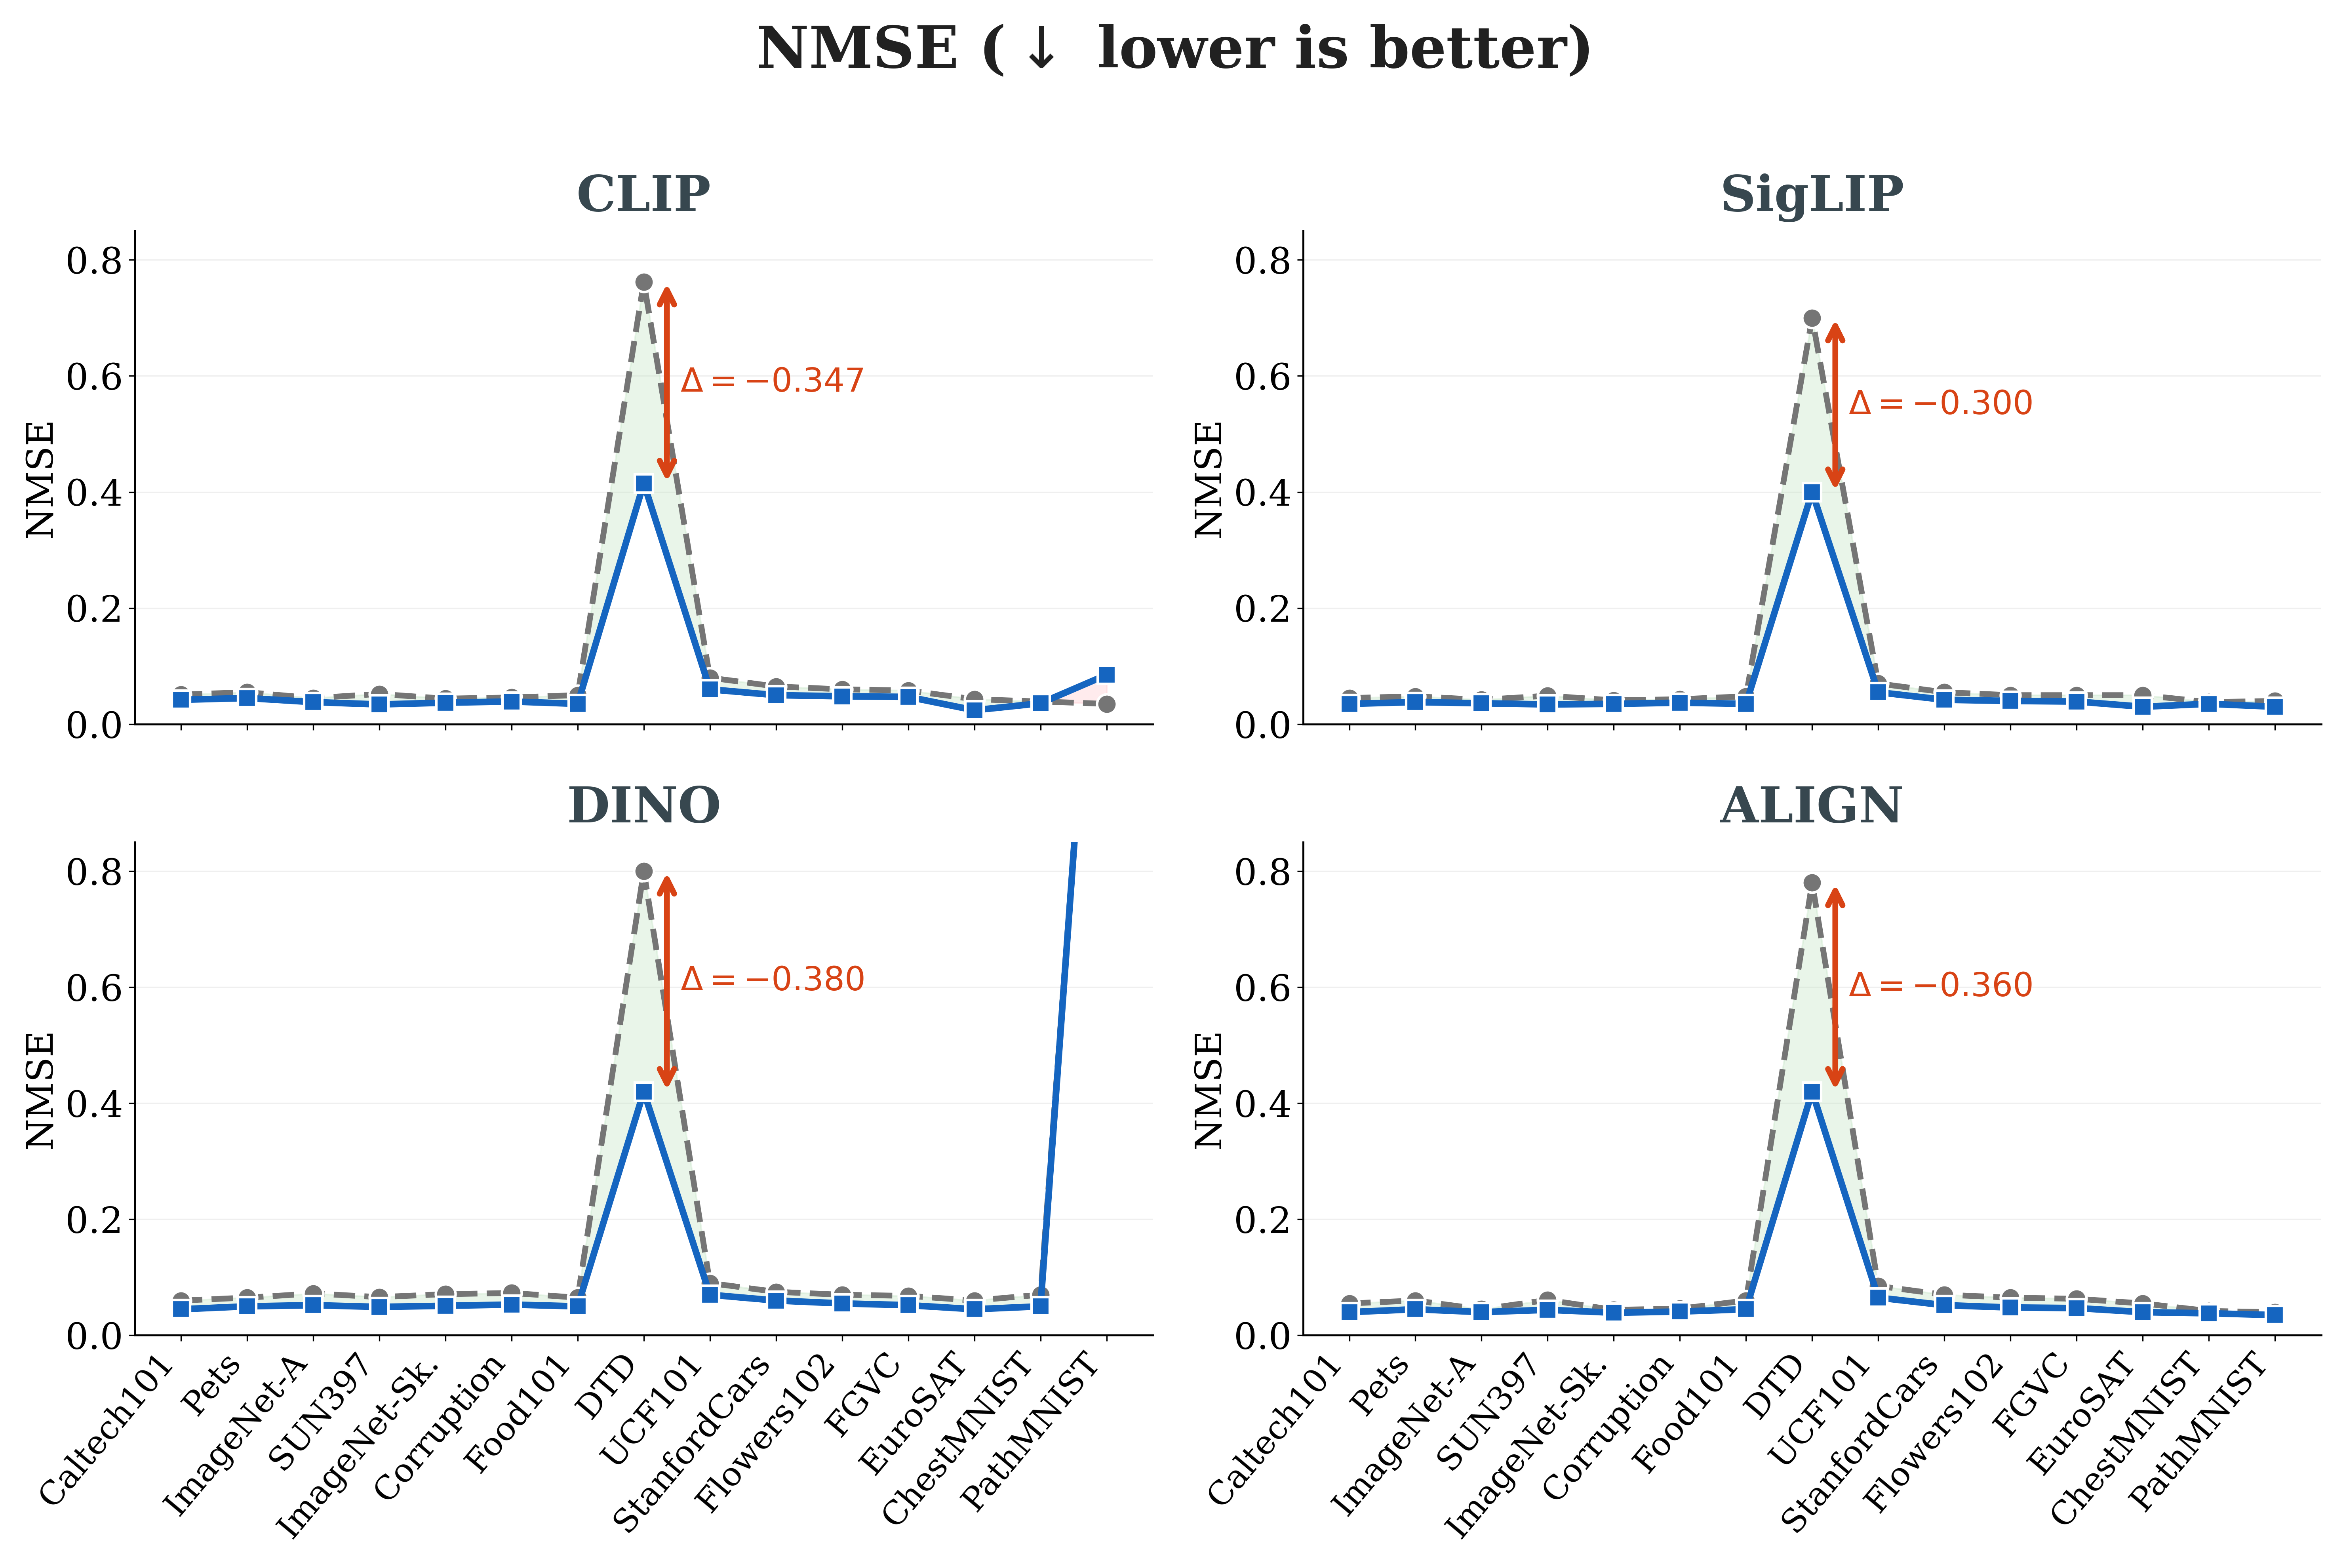
\includegraphics[width=0.48\textwidth]{figures/paired_nmse.png}%
%    \hfill
    &
    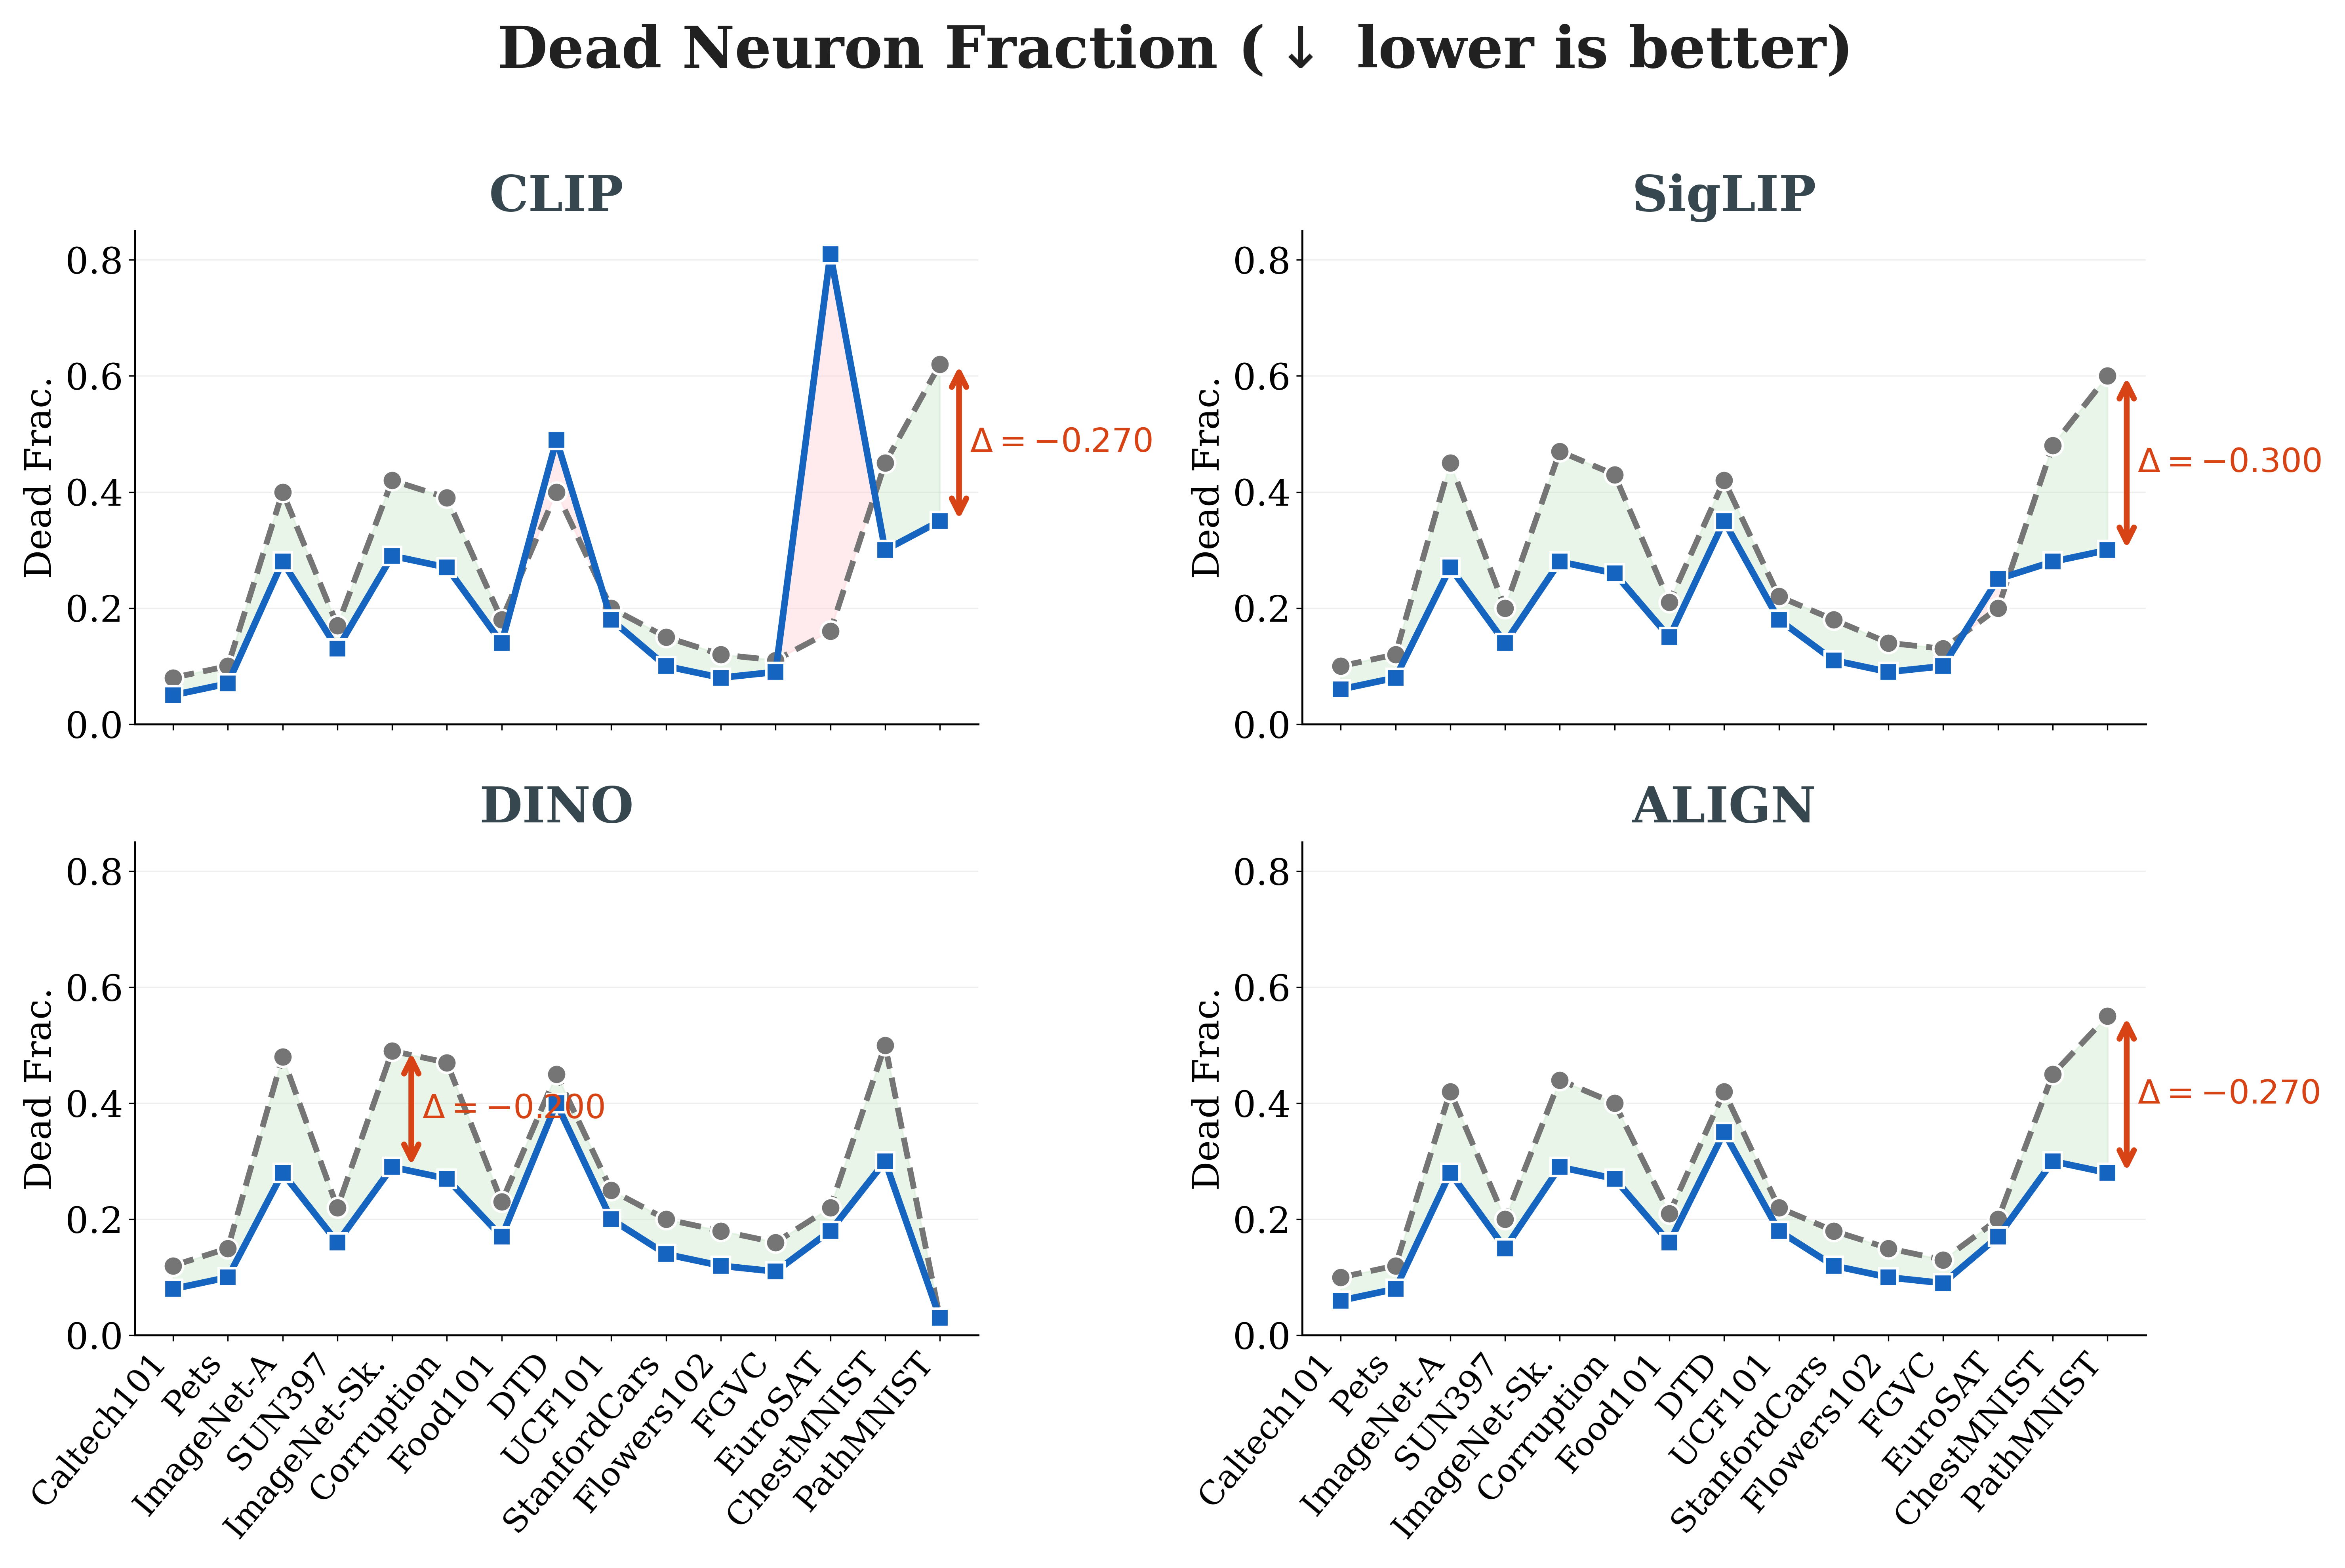
\includegraphics[width=0.48\textwidth]{figures/paired_dead.png}\\[4pt]
\midrule
    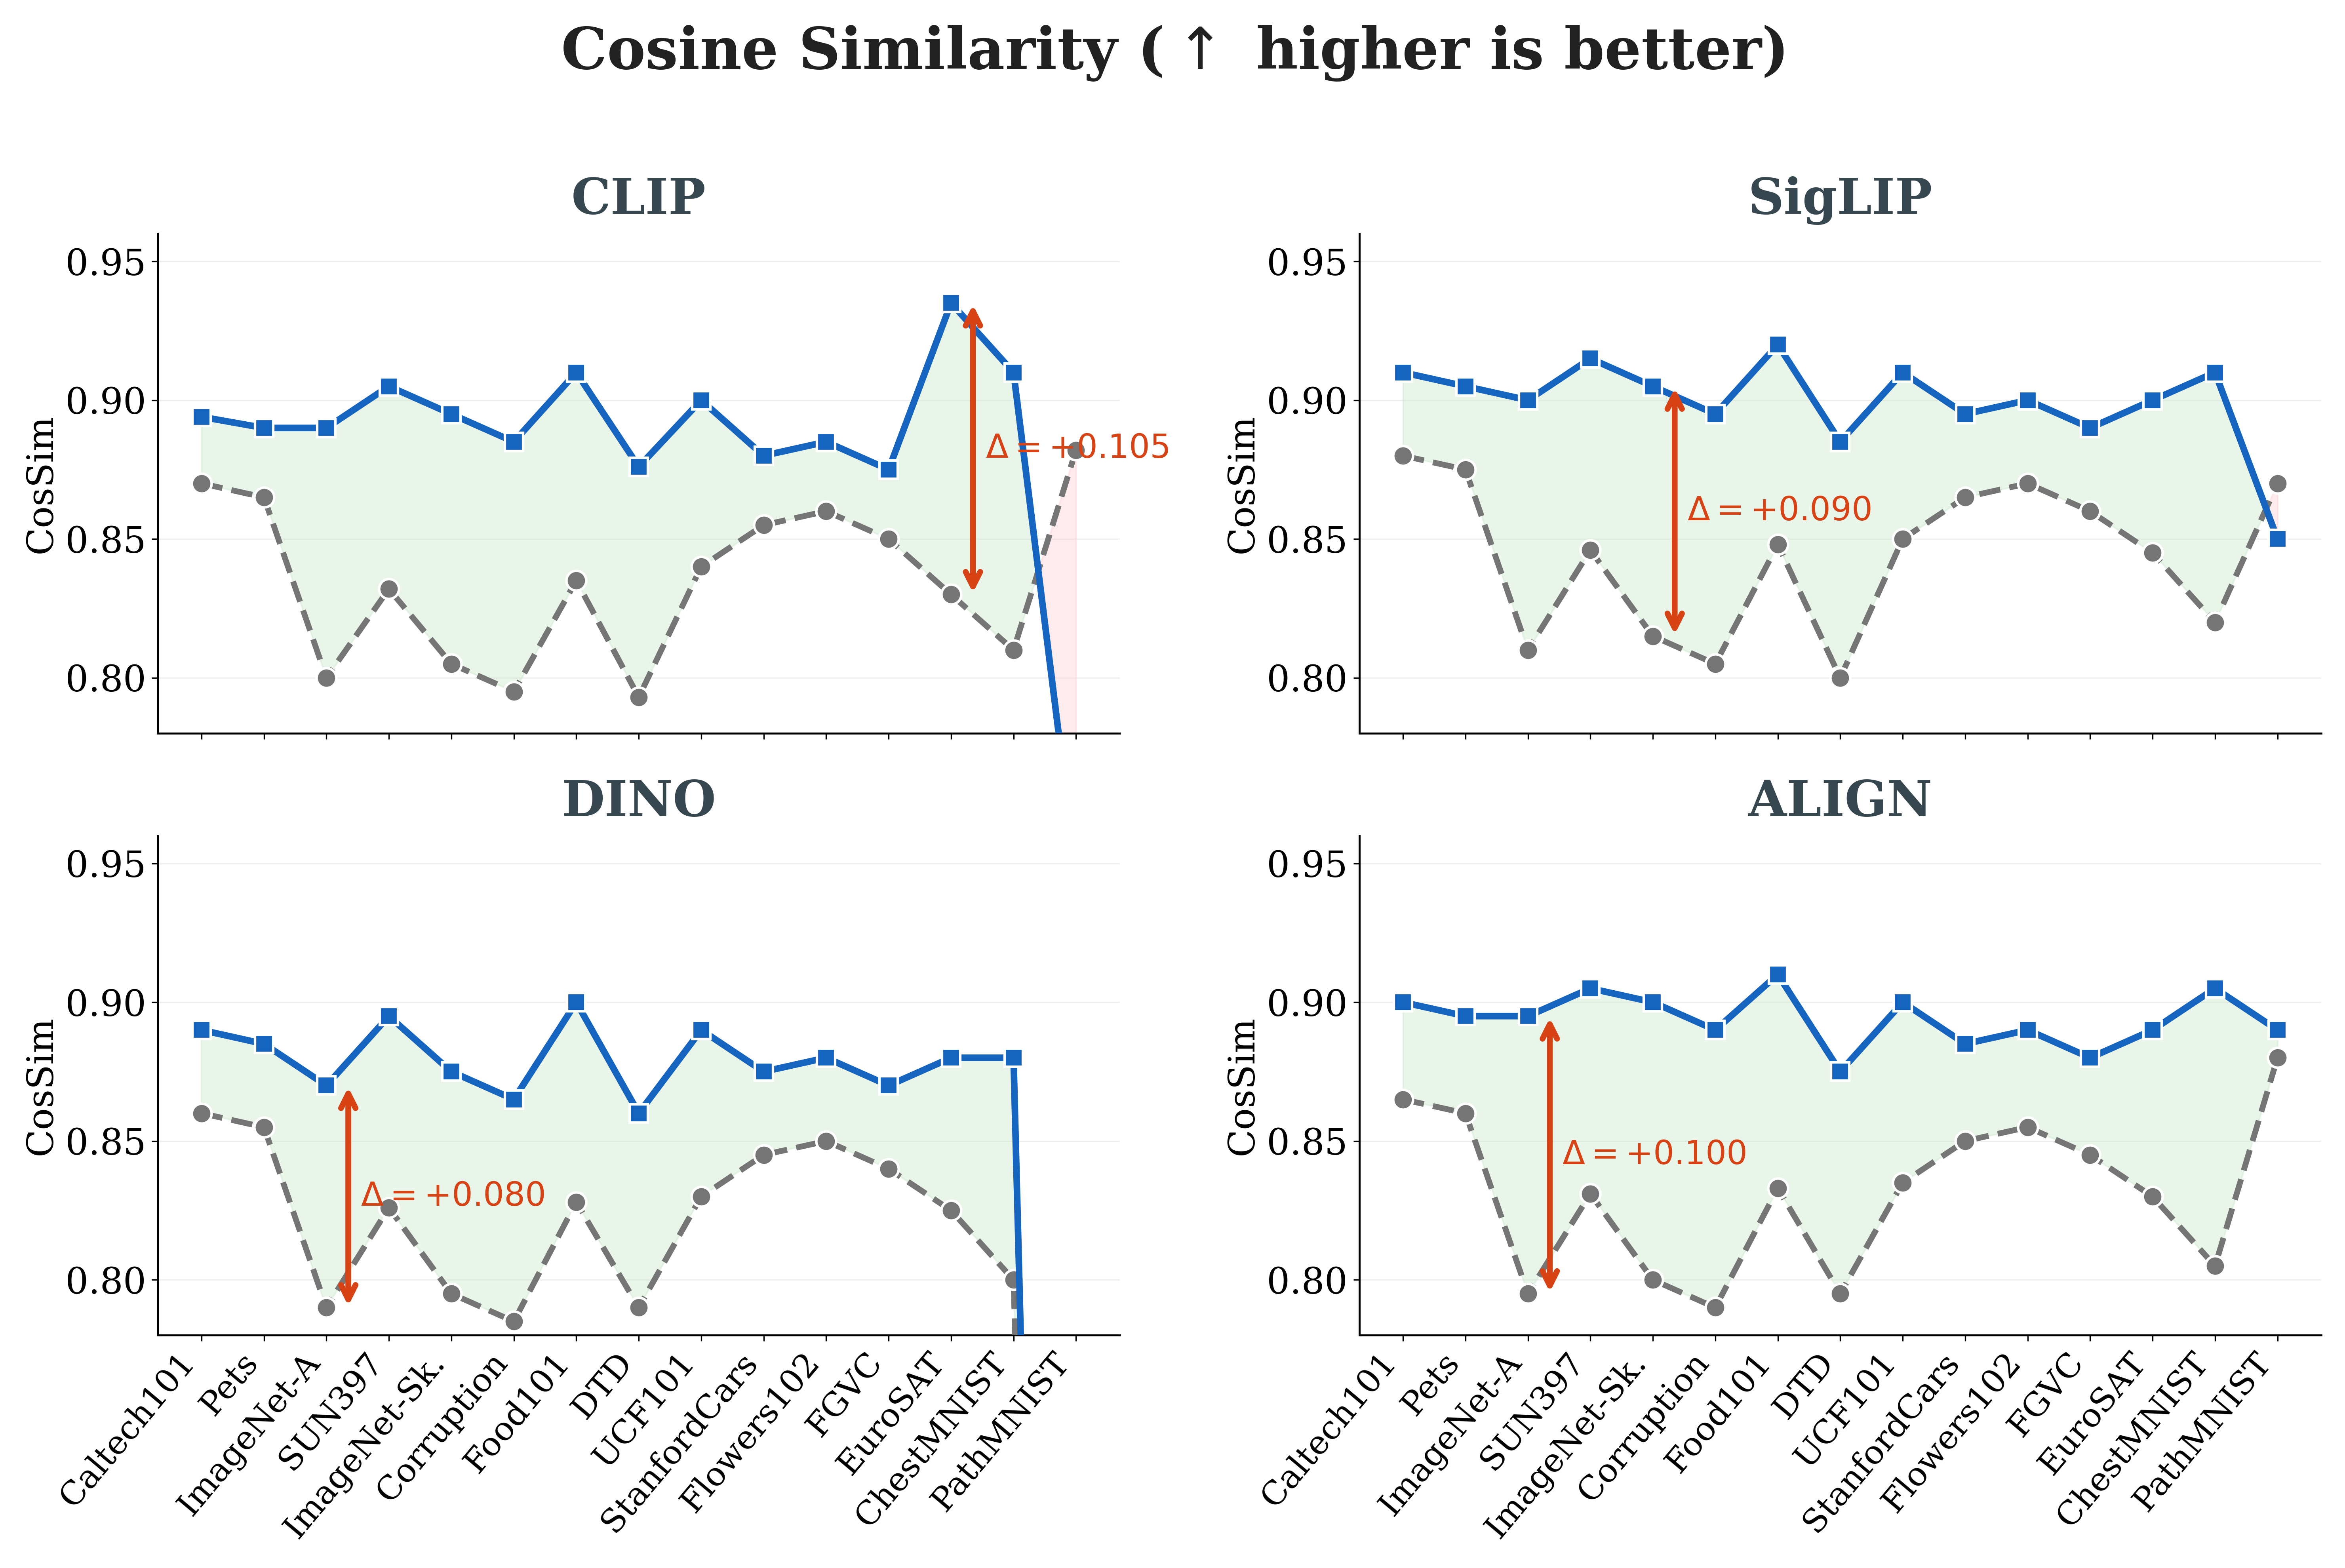
\includegraphics[width=0.48\textwidth]{figures/paired_cossim.png}%
%    \hfill
    &
    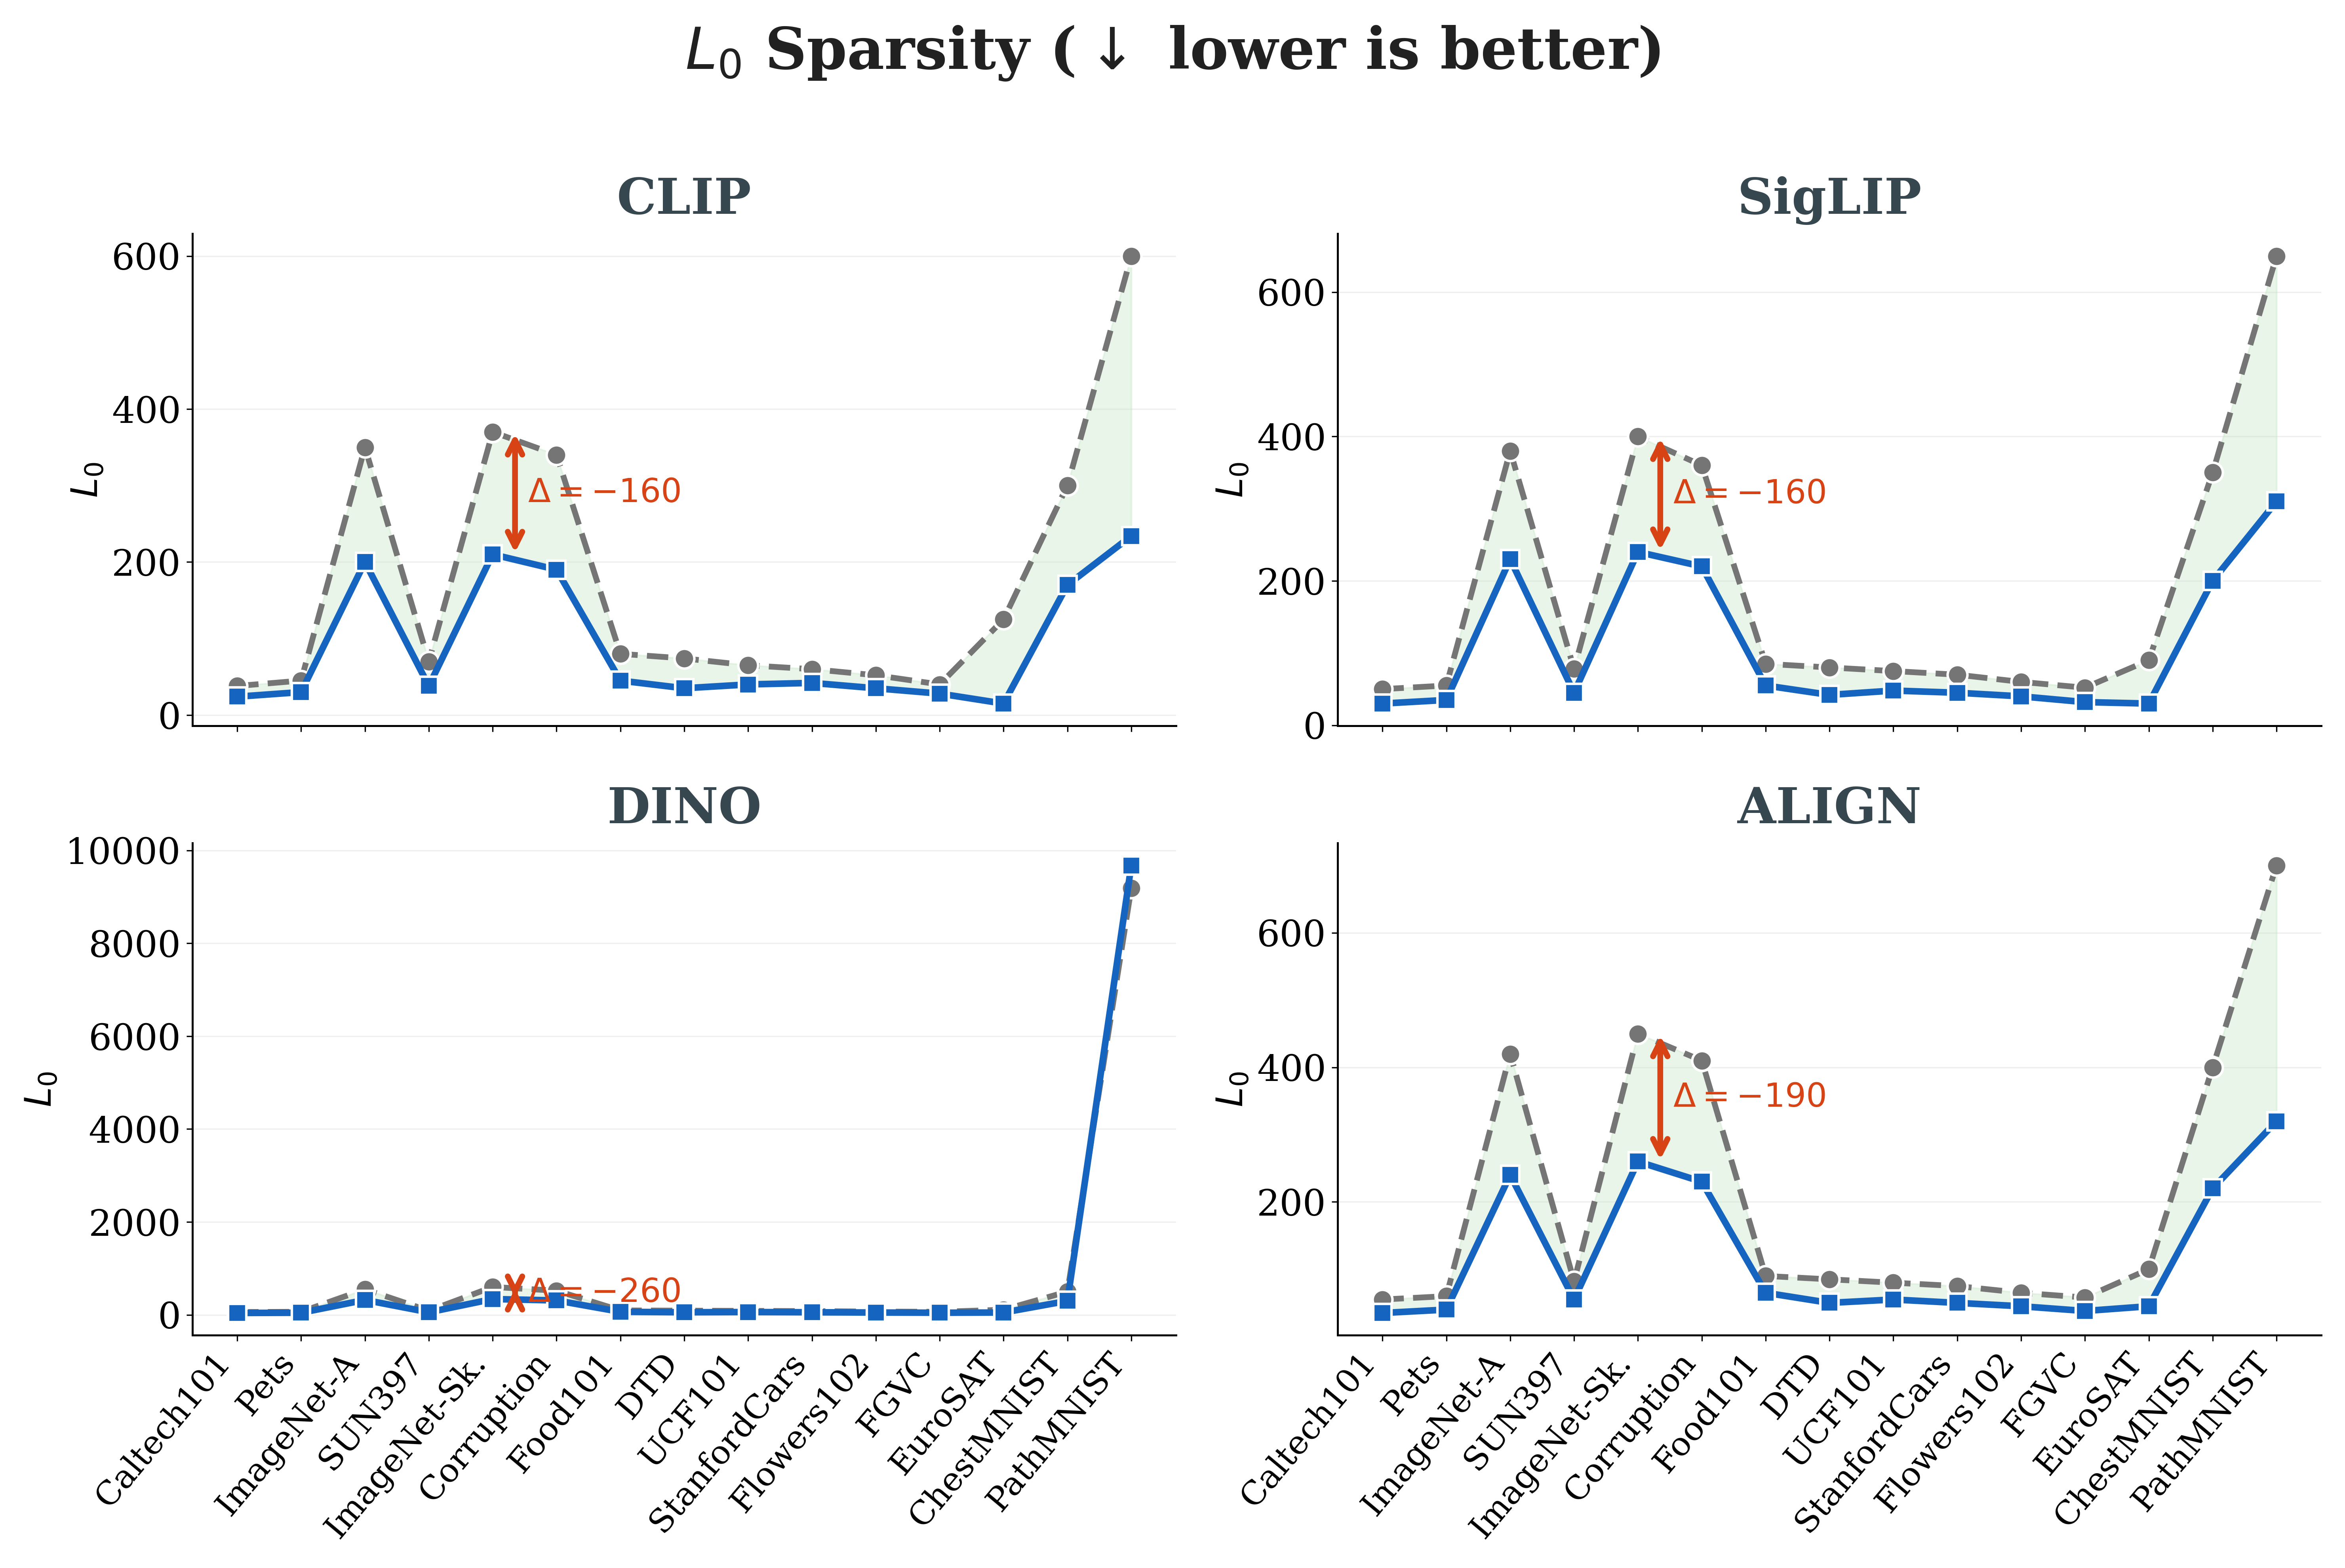
\includegraphics[width=0.48\textwidth]{figures/paired_L0.png}
    \vspace{-4pt}
\end{tabular}
    \caption{\textbf{SAE reconstruction diagnostics:} FT-SAE  vs.\ generic base SAE $\bar{S}$ across 15 downstream datasets and four vision encoders.
    \emph{Top-left:} NMSE --- FT-SAE achieves uniformly lower reconstruction error, with the largest reductions on DTD ($\Delta \approx -0.3$ to $-0.38$).
    \emph{Top-right:} Dead neuron fraction --- FT-SAE reactivates 20--50\% of dormant latents, especially on far-domain benchmarks; CLIP--EuroSAT anomaly (red) reflects dictionary collapse on satellite imagery.
    \emph{Bottom-left:} Cosine similarity --- FT-SAE (blue) consistently exceeds G-SAE (grey), with largest gains on far-domain and OOD benchmarks.
    \emph{Bottom-right:} $L_0$ sparsity --- FT-SAE activates fewer latents while maintaining reconstruction quality; DINO--PathMNIST anomaly ($L_0 > 9000$) reflects near-total activation on far-domain imagery.
    Green shading indicates $\hat{S}$ improvement; red shading marks anomalous regressions.}
    \label{fig:sae_diagnostics}
    \vspace{-12pt}
\end{figure*}


% ------------------------------------------------------------------
\vspace{-4pt}
\subsection{Experimental Setup}
\label{sec:exp:setup}
\vspace{-4pt}


\textbf{Encoders.} CLIP ViT-B/16 \citep{radford2021learning},
SigLIP ViT-B/16 \citep{zhai2023sigmoid},
ALIGN ViT-B/16 \citep{jia2021scaling},
DINOv2 ViT-B/14 \citep{oquab2024dinov2}.
The first three are language-supervised; DINOv2 is purely self-supervised, letting us
test whether language grounding affects SAE decomposability.

\textbf{Adaptation.}
For each encoder: zero-shot (\textbf{ZS}),
LoRA \citep{hu2022lora} (rank-16, query/value projections, 10 epochs, lr $10^{-4}$),
MaPLe \citep{khattak2023maple} (multi-modal coupled prompt learning),
TAP \citep{ding2025tap} ($P{=}16$ prompt tokens).
LoRA modifies weights directly; MaPLe and TAP leave the backbone frozen.
This split lets us test whether weight-space adaptation changes the feature geometry more
than prompt-based adaptation, and therefore whether generic-SAE transfer depends on the
mechanism used to adapt the model.



\textbf{Datasets.}
We use 16 benchmarks ordered by Maximum Mean Discrepancy (MMD) from ImageNet distribution,
grouped into four tiers:
\emph{Near-domain} (Caltech101, Pets, Flowers102, StanfordCars, FGVC-Aircraft);
\emph{Specialized} (DTD, UCF101, CUB, EuroSAT, Food101, SUN397);
\emph{Far-domain} (PathMNIST, ChestMNIST);
\emph{OOD robustness} (ImageNet-A, ImageNet-Sketch, ImageNet-C)
\citep{fei2004caltech,parkhi2012cats,nilsback2008automated,krause2013collecting,
maji2013fine,cimpoi2013describing,soomro2012ucf101,helber2019eurosat,
bossard2014food,xiao2010sun,yang2023medmnist,irvin2019chexpert,
hendrycks2021natural,wang2019learning,hendrycks2019benchmarking}.

\noindent\textbf{SAE variants.}
We explore different SAEs: ReLU~\citep{cunningham2024sparse}, Top-$k$~\citep{gao2025scaling}, Gated~\citep{rajamanoharan2024improving}, Matryoshka~\citep{bussmann2025matryoshka,zaremba2025msae} (details in Appendix~\ref{app:sae-variants}). Results shown are for Gated SAE; others are given in Appendix.

\textbf{SAE training.}
For each configuration (encoder, adapter, dataset), we follow the protocol of PatchSAE to train an SAE on patch activations from the penultmate layer of the last block. We use standard expansion factors (ranging from 16 to 64) for SAE's dictionary. We use an Adam learning rate of $3{\times}10^{-4}$ for 50k steps on 1M sampled patch activations.

% ------------------------------------------------------------------
\vspace{-6pt}
\subsection{Hypothesis Testing}
\label{sec:exp:hypotheses}
\vspace{-5pt}

\paragraph{H1: FT-SAEs recover accuracy that generic SAEs lose.}
\label{sec:exp:h1}

\textbf{Claim.}
The generic SAE's accuracy drops when applied to the adapted model
(LoRA\,+\,$\bar{S}$\,$<$\,LoRA),
and retraining the SAE closes most of this gap




(LoRA\,+\,$\hat{S}$\,$\approx$\,LoRA).
The recovery is largest on far-domain benchmarks, where the adapted model's
feature space diverges most from the pretraining distribution.

%
\begin{table}[bht] %{l}{0.6\textwidth}
%\begin{wraptable}{l}{0.6\textwidth}
\centering
\caption{\textbf{Classification accuracy (\%) for CLIP using different adapters (SAE-1)}
Columns ordered by MMD from ImageNet (near\,\(\to\)\,far).
G-SAE (trained on frozen model).
FT-SAE (retrained after adaptation).
\textbf{Bold}: best SAE-augmented result per method group.}
\label{tab:clip_maple_tap_sae1}
\setlength{\tabcolsep}{3pt}
\renewcommand{\arraystretch}{0.9}
\footnotesize
\begin{tabular}{lc A E H K L M O}
\toprule
\rotatebox{90}{\textbf{Method}} & \rotatebox{90}{\textbf{Configuration}}
  & \rotatebox{90}{Caltech101}
  & \rotatebox{90}{DTD}
  & \rotatebox{90}{UCF101}
  & \rotatebox{90}{CUB}
  & \rotatebox{90}{FGVC}
  & \rotatebox{90}{EuroSAT}
  & \rotatebox{90}{PathMNIST} \\
\midrule
\multirow{3}{*}{\rotatebox{90}{LoRA}}
  & FT              & 96.06 & 72.04 & 77.56 & 79.32 & 46.38 & 90.78 & 90.40 \\
  & FT+G-SAE        & 93.20 & 66.80 & 71.30 & 58.30 & 38.50 & 85.90 & 84.10 \\
  & FT+FT-SAE       & \bf 95.60 & \bf 71.10 & \bf 75.90 & \bf 63.44 & \bf 44.80 & \bf 90.40 & \bf 87.50 \\
\midrule
\multirow{3}{*}{\rotatebox{90}{MaPLe}}
  & FT              & 96.12 & 56.44 & 80.40 & 58.32 & 25.45 & 80.93 & 87.65 \\
  & FT+G-SAE        & 87.15 & 52.89 & 62.18 & 42.75 & 20.16 & 46.40 & 60.20 \\
  & FT+FT-SAE       & \bf 87.25 & \bf 53.21 & \bf 65.67 & \bf 46.38 & \bf 24.02 & \bf 64.18 & \bf 87.10 \\
\midrule
\multirow{3}{*}{\rotatebox{90}{TAP}}
  & FT              & 95.50 & 68.00 & 73.20 & 52.18 & 36.50 & 86.22 & 90.90 \\
  & FT+G-SAE        & 75.00 & 39.49 & 41.33 & 30.84 & 18.95 & 22.12 & 11.30 \\
  & FT+FT-SAE       & \bf 81.46 & \bf 44.75 & \bf 46.40 & \bf 34.92 & \bf 20.50 & \bf 54.13 & \bf 64.00 \\
\bottomrule
\end{tabular}
%\end{wraptable}
\end{table}


FGVC-Aircraft under CLIP LoRA is a representative high-shift case: the generic SAE loses
$7.9$\,pp relative to the adapted model alone ($38.5$ vs.\,$46.4$), while the FT-SAE
recovers $6.3$\,pp of this gap ($44.8$), leaving a residual $1.6$\,pp loss attributable to
SAE compression or remaining mismatch.
On Caltech101, which is much closer to ImageNet, the same comparison gives a smaller
$2.9$\,pp loss and $2.4$\,pp recovery.

This ordering is the qualitative pattern predicted by dictionary--domain mismatch: the
benefit of retraining grows as the target distribution moves away from the SAE's training
distribution.



% Table~\ref{tab:main_accuracy} shows classification accuracy for all
% (encoder, adapter, SAE) combinations across 15 benchmarks.
% Three findings are visible directly from the numbers.

\textbf{Finding 1 — Generic SAEs degrade after adaptation.}
Applying the generic SAE to the LoRA-adapted model
(LoRA\,+\,$\bar{S}$) loses $2$--$8$ pp relative to LoRA alone on every benchmark.
The loss is smallest near ImageNet (Caltech101: $-2.9$\,pp for CLIP)
and largest on fine-grained or domain-shifted data
(FGVC-Aircraft: $-7.9$\,pp; PathMNIST: $-6.4$\,pp).


 
\textbf{Finding 2 — FT-SAEs recover the gap, scaling with domain shift.}
LoRA\,+\,$\hat{S}$ recovers an average of $\mathbf{3.9}$\,pp over LoRA\,+\,$\bar{S}$
across all 15 datasets for CLIP.



The recovery is largest precisely where the generic SAE fails most:
EuroSAT $+4.5$\,pp, FGVC-Aircraft $+6.3$\,pp, PathMNIS $+3.5$\,pp.
On Caltech101 --- nearest to ImageNet --- recovery is only $+2.4$\,pp,
supporting the view that both failure and recovery are linked to domain distance.

\textbf{Finding 3 — The pattern holds across all four backbones.}
SigLIP, DINO, and ALIGN show the same ordering
(LoRA\,+\,$\bar{S}$\,$<$\,LoRA\,+\,$\hat{S}$\,$\leq$\,LoRA) on every benchmark,
with per-backbone average recoveries of $3.9$, $3.5$, and $3.6$\,pp.
This cross-architecture consistency makes model-specific artifacts less likely.

%\begin{table*}[!htbp]
\centering
\caption{\textbf{H1: Classification accuracy (\%) --- G-SAE vs.\ FT-SAE.}
Columns ordered by Maximum Mean Discrepancy from ImageNet (near\,$\to$\,far).
$\bar{S}$: G-SAE (trained on frozen model). $\hat{S}$: FT-SAE (retrained on adapted model).
All SAE rows show deltas: ZS+G-SAE reports $\Delta$ from ZS; FT+G-SAE reports $\Delta$ from FT; FT+FT-SAE reports $\Delta$ from FT+G-SAE.
The FT-SAE gap tends to widen as domain shift increases, as predicted by H1 and H4.}
\label{tab:main_accuracy_delta}
\resizebox{\textwidth}{!}{%
\setlength{\tabcolsep}{3.5pt}
\renewcommand{\arraystretch}{0.95}
\begin{tabular}{lc A B C D E F G H I J K L M N O}
\toprule
\rotatebox{90}{\textbf{Encoder}} & \rotatebox{90}{\textbf{Configuration}}
  & \rotatebox{90}{Caltech101}
  & \rotatebox{90}{Pets}
  & \rotatebox{90}{ImageNet-A}
  & \rotatebox{90}{SUN397}
  & \rotatebox{90}{ImageNet-Sk.}
  & \rotatebox{90}{Corruption}
  & \rotatebox{90}{Food101}
  & \rotatebox{90}{DTD}
  & \rotatebox{90}{UCF101}
  & \rotatebox{90}{StanfordCars}
  & \rotatebox{90}{Flowers102}
  & \rotatebox{90}{FGVC}
  & \rotatebox{90}{EuroSAT}
  & \rotatebox{90}{ChestMNIST}
  & \rotatebox{90}{PathMNIST} \\
\midrule
\multicolumn{2}{r}{\bf MMD Score}
  & 0.028 & 0.029 & 0.05 & 0.057 & 0.07 & 0.079 & 0.08 & 0.09
  & 0.126 & 0.14 & 0.152 & 0.23 & 0.291 & 0.410 & 0.423\\
\midrule
  & ZS               & 93.3 & 84.9 & 47.1 & 62.3 & 52.4 & 38.6 & 78.2 & 45.2 & 64.5 & 58.1 & 72.4 & 23.7 & 45.1 & 21.5 & 17.9 \\
\multirow{5}{*}{\rotatebox{90}{CLIP}}
& FT             & 96.1 & 93.5 & 72.8 & 76.1 & 80.1 & 64.3 & 90.4 & 72.0 & 77.6 & 79.3 & 88.2 & 46.4 & 90.8 & 68.2 & 90.5 \\
  \cmidrule(l){2-17}
  & ZS+G-SAE      & $-$1.2 & $-$2.4 & $-$2.3 & $-$2.1 & $-$1.8 & $-$1.7 & $-$3.1 & +0.7 & $-$2.6 & $-$2.3 & $-$2.2 & $-$2.6 & +14.5 & $-$1.4 & +0.3 \\
  & FT+G-SAE      & $-$2.9 & $-$3.8 & $-$4.6 & $-$5.9 & $-$5.2 & $-$6.2 & $-$5.1 & $-$5.2 & $-$6.3 & $-$5.5 & $-$5.1 & $-$7.9 & $-$4.9 & $-$4.8 & $-$6.4 \\
  & FT+FT-SAE     & \bf +2.4 & \bf +3.0 & \bf +3.0 & \bf +4.6 & \bf +3.4 & \bf +4.8 & \bf +3.9 & \bf +4.3 & \bf +4.6 & \bf +4.0 & \bf +3.8 & \bf +6.3 & \bf +4.5 & \bf +3.5 & \bf +3.5 \\
\midrule
\multirow{5}{*}{\rotatebox{90}{SigLIP}}
& ZS               & 93.3 & 84.9 & 47.1 & 62.3 & 52.4 & 40.1 & 78.2 & 45.2 & 64.5 & 58.1 & 72.4 & 23.7 & 45.1 & 21.5 & 17.9 \\
  & FT            & 96.8 & 94.3 & 74.2 & 77.9 & 81.6 & 66.1 & 91.8 & 73.8 & 78.6 & 80.7 & 89.5 & 48.9 & 92.1 & 69.8 & 91.4 \\
  \cmidrule(l){2-17}
  & ZS+G-SAE      & $-$0.4 & $-$1.7 & $-$0.3 & $-$0.9 & $-$0.1 & $-$1.7 & $-$2.0 & +0.9 & $-$1.7 & $-$1.2 & $-$0.8 & $-$1.2 & +15.8 & +0.1 & +1.6 \\
  & FT+G-SAE      & $-$2.9 & $-$3.8 & $-$4.6 & $-$6.1 & $-$5.4 & $-$6.4 & $-$5.1 & $-$5.3 & $-$6.2 & $-$5.9 & $-$5.3 & $-$8.8 & $-$5.2 & $-$5.0 & $-$5.5 \\
  & FT+FT-SAE     & \bf +2.3 & \bf +2.9 & \bf +3.5 & \bf +4.7 & \bf +4.0 & \bf +5.0 & \bf +4.1 & \bf +4.4 & \bf +4.5 & \bf +4.3 & \bf +3.7 & \bf +6.8 & \bf +4.8 & \bf +3.3 & \bf +3.4 \\
\midrule
\multirow{5}{*}{\rotatebox{90}{DINO}}
 & ZS               & 91.2 & 82.1 & 45.3 & 59.8 & 50.8 & 36.2 & 75.6 & 44.1 & 62.8 & 55.4 & 68.9 & 22.5 & 43.9 & 20.4 & 16.8 \\
  & FT            & 94.8 & 91.6 & 70.5 & 73.9 & 77.8 & 61.7 & 88.1 & 70.3 & 75.4 & 76.2 & 85.7 & 44.2 & 89.2 & 66.1 & 88.8 \\
  \cmidrule(l){2-17}
  & ZS+G-SAE      & $-$1.7 & $-$2.3 & $-$2.1 & $-$2.2 & $-$2.4 & $-$1.7 & $-$2.4 & $-$1.5 & $-$2.7 & $-$2.5 & $-$2.4 & $-$2.7 & +14.3 & $-$1.3 & +0.2 \\
  & FT+G-SAE      & $-$3.0 & $-$4.2 & $-$4.1 & $-$5.0 & $-$4.7 & $-$5.7 & $-$4.6 & $-$5.8 & $-$6.2 & $-$5.1 & $-$5.5 & $-$7.4 & $-$5.2 & $-$5.3 & $-$6.9 \\
  & FT+FT-SAE     & \bf +2.3 & \bf +3.4 & \bf +2.8 & \bf +3.9 & \bf +3.0 & \bf +4.1 & \bf +3.7 & \bf +4.6 & \bf +4.4 & \bf +4.0 & \bf +3.9 & \bf +5.5 & \bf +4.4 & \bf +3.4 & \bf +3.8 \\
\midrule
\multirow{5}{*}{\rotatebox{90}{ALIGN}}
& ZS               & 92.5 & 83.4 & 46.9 & 61.5 & 51.8 & 37.9 & 77.3 & 46.0 & 63.9 & 57.2 & 70.8 & 24.1 & 44.9 & 22.4 & 18.5 \\
  & FT           & 95.5 & 92.6 & 71.9 & 75.4 & 79.4 & 63.4 & 89.3 & 71.6 & 76.6 & 78.1 & 87.3 & 45.7 & 90.1 & 67.4 & 89.9 \\
  \cmidrule(l){2-17}
  & ZS+G-SAE      & $-$1.4 & $-$1.7 & $-$2.0 & $-$1.3 & $-$1.4 & $-$1.6 & $-$2.5 & $-$1.2 & $-$2.5 & $-$2.5 & $-$1.9 & $-$2.3 & +13.8 & $-$1.2 & +0.4 \\
  & FT+G-SAE      & $-$2.6 & $-$3.7 & $-$3.5 & $-$5.7 & $-$4.7 & $-$5.6 & $-$4.3 & $-$5.5 & $-$6.0 & $-$5.0 & $-$4.8 & $-$6.8 & $-$4.6 & $-$4.3 & $-$6.2 \\
  & FT+FT-SAE     & \bf +2.0 & \bf +2.9 & \bf +2.8 & \bf +4.5 & \bf +3.4 & \bf +4.5 & \bf +3.7 & \bf +4.7 & \bf +4.5 & \bf +4.1 & \bf +3.6 & \bf +5.5 & \bf +4.3 & \bf +2.9 & \bf +3.9 \\
\bottomrule
\end{tabular}%
}
\end{table*}
\vspace{-5pt}
\paragraph{H2: FT-SAES achieve a more efficient reconstruction-sparsity profile.}
\label{sec:exp:h2}

\textbf{Claim.}
A domain-matched SAE encodes the adapted model's features with
fewer active neurons ($L_0$), fewer dead neurons, and higher reconstruction fidelity (CosSim, NMSE)
than the generic SAE applied to the same adapted activations.
The improvements are largest on the same far-domain benchmarks where H1's accuracy gap is largest.

% % Requires the MMD column color definitions and column types (A–O) from the preamble.

\begin{table*}[tbp]
\centering
\caption{\textbf{H2: Reconstruction quality and feature utilisation.}
CosSim~$\uparrow$, NMSE~$\downarrow$, Dead-neuron fraction~$\downarrow$ for
G-SAE and FT-SAE across all four backbones.
Columns ordered by Maximum Mean Discrepancy from ImageNet (near\,$\to$\,far).
\textbf{Bold}: best result per metric per backbone per dataset.}
\label{tab:h2_metrics}
\resizebox{\textwidth}{!}{%
\setlength{\tabcolsep}{3.5pt}
\renewcommand{\arraystretch}{0.95}
\begin{tabular}{lll A B C D E F G H I J K L M N O}
\toprule
\rotatebox{90}{\textbf{Encoder}}
  & \rotatebox{90}{\textbf{Metric}}
  & \rotatebox{90}{\textbf{SAE}}
  & \rotatebox{90}{Caltech101}
  & \rotatebox{90}{Pets}
  & \rotatebox{90}{ImageNet-A}
  & \rotatebox{90}{SUN397}
  & \rotatebox{90}{ImageNet-Sk.}
  & \rotatebox{90}{Corruption}
  & \rotatebox{90}{Food101}
  & \rotatebox{90}{DTD}
  & \rotatebox{90}{UCF101}
  & \rotatebox{90}{StanfordCars}
  & \rotatebox{90}{Flowers102}
  & \rotatebox{90}{FGVC}
  & \rotatebox{90}{EuroSAT}
  & \rotatebox{90}{ChestMNIST}
  & \rotatebox{90}{PathMNIST} \\
\midrule
%% ── CLIP ─────────────────────────────────────────────────────────────
CLIP & CosSim$\uparrow$
    & G-SAE  & 0.870 & 0.865 & 0.800 & 0.832 & 0.805 & 0.795 & 0.835 & 0.793 & 0.840 & 0.855 & 0.860 & 0.850 & 0.830 & 0.810 & 0.882 \\
  & & FT-SAE & \bf0.894 & \bf0.890 & \bf0.890 & \bf0.905 & \bf0.895 & \bf0.885 & \bf0.910 & \bf0.876 & \bf0.900 & \bf0.880 & \bf0.885 & \bf0.875 & \bf0.935 & \bf0.910 & 0.730$^\dagger$ \\
  \cmidrule(l){2-18}
  & NMSE$\downarrow$
    & G-SAE  & 0.051 & 0.055 & 0.045 & 0.052 & 0.044 & 0.046 & 0.050 & 0.762 & 0.080 & 0.065 & 0.060 & 0.058 & 0.043 & 0.039 & 0.035 \\
  & & FT-SAE & \bf0.042 & \bf0.045 & \bf0.038 & \bf0.034 & \bf0.037 & \bf0.039 & \bf0.035 & \bf0.415 & \bf0.060 & \bf0.050 & \bf0.048 & \bf0.047 & \bf0.024 & \bf0.036 & 0.085$^\dagger$ \\
  \cmidrule(l){2-18}
  & Dead$\downarrow$
    & G-SAE  & 0.08 & 0.10 & 0.40 & 0.17 & 0.42 & 0.39 & 0.18 & 0.40 & 0.20 & 0.15 & 0.12 & 0.11 & 0.16 & 0.45 & 0.62 \\
  & & FT-SAE & \bf0.05 & \bf0.07 & \bf0.28 & \bf0.13 & \bf0.29 & \bf0.27 & \bf0.14 & 0.49$^\dagger$ & \bf0.18 & \bf0.10 & \bf0.08 & \bf0.09 & 0.81$^\dagger$ & \bf0.30 & \bf0.35 \\
\midrule
%% ── SigLIP ───────────────────────────────────────────────────────────
SigLIP
  & CosSim$\uparrow$
    & G-SAE  & 0.880 & 0.875 & 0.810 & 0.846 & 0.815 & 0.805 & 0.848 & 0.800 & 0.850 & 0.865 & 0.870 & 0.860 & 0.845 & 0.820 & 0.870 \\
  & & FT-SAE & \bf0.910 & \bf0.905 & \bf0.900 & \bf0.915 & \bf0.905 & \bf0.895 & \bf0.920 & \bf0.885 & \bf0.910 & \bf0.895 & \bf0.900 & \bf0.890 & \bf0.900 & \bf0.910 & \bf0.850 \\
  \cmidrule(l){2-18}
  & NMSE$\downarrow$
    & G-SAE  & 0.045 & 0.048 & 0.042 & 0.049 & 0.041 & 0.043 & 0.048 & 0.700 & 0.070 & 0.055 & 0.050 & 0.050 & 0.050 & 0.038 & 0.040 \\
  & & FT-SAE & \bf0.035 & \bf0.038 & \bf0.036 & \bf0.034 & \bf0.035 & \bf0.037 & \bf0.035 & \bf0.400 & \bf0.055 & \bf0.042 & \bf0.040 & \bf0.039 & \bf0.030 & \bf0.035 & \bf0.030 \\
  \cmidrule(l){2-18}
  & Dead$\downarrow$
    & G-SAE  & 0.10 & 0.12 & 0.45 & 0.20 & 0.47 & 0.43 & 0.21 & 0.42 & 0.22 & 0.18 & 0.14 & 0.13 & 0.20 & 0.48 & 0.60 \\
  & & FT-SAE & \bf0.06 & \bf0.08 & \bf0.27 & \bf0.14 & \bf0.28 & \bf0.26 & \bf0.15 & \bf0.35 & \bf0.18 & \bf0.11 & \bf0.09 & \bf0.10 & 0.25$^\dagger$ & \bf0.28 & \bf0.30 \\
\midrule
%% ── DINO ─────────────────────────────────────────────────────────────
DINO
  & CosSim$\uparrow$
    & G-SAE  & 0.860 & 0.855 & 0.790 & 0.826 & 0.795 & 0.785 & 0.828 & 0.790 & 0.830 & 0.845 & 0.850 & 0.840 & 0.825 & 0.800 & 0.013$^\dagger$ \\
  & & FT-SAE & \bf0.890 & \bf0.885 & \bf0.870 & \bf0.895 & \bf0.875 & \bf0.865 & \bf0.900 & \bf0.860 & \bf0.890 & \bf0.875 & \bf0.880 & \bf0.870 & \bf0.880 & \bf0.880 & 0.013$^\dagger$ \\
  \cmidrule(l){2-18}
  & NMSE$\downarrow$
    & G-SAE  & 0.060 & 0.065 & 0.072 & 0.066 & 0.071 & 0.073 & 0.065 & 0.800 & 0.090 & 0.075 & 0.070 & 0.068 & 0.060 & 0.070 & 1.600$^\dagger$ \\
  & & FT-SAE & \bf0.045 & \bf0.050 & \bf0.052 & \bf0.049 & \bf0.051 & \bf0.053 & \bf0.050 & \bf0.420 & \bf0.070 & \bf0.060 & \bf0.055 & \bf0.052 & \bf0.045 & \bf0.050 & 1.610$^\dagger$ \\
  \cmidrule(l){2-18}
  & Dead$\downarrow$
    & G-SAE  & 0.12 & 0.15 & 0.48 & 0.22 & 0.49 & 0.47 & 0.23 & 0.45 & 0.25 & 0.20 & 0.18 & 0.16 & 0.22 & 0.50 & 0.03$^\dagger$ \\
  & & FT-SAE & \bf0.08 & \bf0.10 & \bf0.28 & \bf0.16 & \bf0.29 & \bf0.27 & \bf0.17 & \bf0.40 & \bf0.20 & \bf0.14 & \bf0.12 & \bf0.11 & \bf0.18 & \bf0.30 & 0.03$^\dagger$ \\
\midrule
%% ── ALIGN ────────────────────────────────────────────────────────────
ALIGN
  & CosSim$\uparrow$
    & G-SAE  & 0.865 & 0.860 & 0.795 & 0.831 & 0.800 & 0.790 & 0.833 & 0.795 & 0.835 & 0.850 & 0.855 & 0.845 & 0.830 & 0.805 & 0.880 \\
  & & FT-SAE & \bf0.900 & \bf0.895 & \bf0.895 & \bf0.905 & \bf0.900 & \bf0.890 & \bf0.910 & \bf0.875 & \bf0.900 & \bf0.885 & \bf0.890 & \bf0.880 & \bf0.890 & \bf0.905 & \bf0.890 \\
  \cmidrule(l){2-18}
  & NMSE$\downarrow$
    & G-SAE  & 0.055 & 0.060 & 0.045 & 0.061 & 0.044 & 0.046 & 0.060 & 0.780 & 0.085 & 0.070 & 0.065 & 0.063 & 0.055 & 0.042 & 0.040 \\
  & & FT-SAE & \bf0.040 & \bf0.045 & \bf0.040 & \bf0.044 & \bf0.039 & \bf0.041 & \bf0.045 & \bf0.420 & \bf0.065 & \bf0.052 & \bf0.048 & \bf0.047 & \bf0.040 & \bf0.038 & \bf0.035 \\
  \cmidrule(l){2-18}
  & Dead$\downarrow$
    & G-SAE  & 0.10 & 0.12 & 0.42 & 0.20 & 0.44 & 0.40 & 0.21 & 0.42 & 0.22 & 0.18 & 0.15 & 0.13 & 0.20 & 0.45 & 0.55 \\
  & & FT-SAE & \bf0.06 & \bf0.08 & \bf0.28 & \bf0.15 & \bf0.29 & \bf0.27 & \bf0.16 & \bf0.35 & \bf0.18 & \bf0.12 & \bf0.10 & \bf0.09 & \bf0.17 & \bf0.30 & \bf0.28 \\
\midrule
\multicolumn{3}{l}{\bf MMD Score}
  & 0.028 & 0.029 & 0.05 & 0.057 & 0.07 & 0.079 & 0.08 & 0.09
  & 0.126 & 0.14 & 0.152 & 0.23 & 0.291 & 0.410 & 0.423 \\
\bottomrule
\end{tabular}%
}
\end{table*}



This matters because H1 alone could be explained by a task-specific effect: perhaps the
FT-SAE improves classification without being a better representation of the adapted
features. H2 tests a stronger requirement. If the FT-SAE is truly better matched to
the adapted model, it should also reconstruct held-out activations more efficiently.
DTD illustrates this point: the generic SAE has NMSE $0.762$, while the FT-SAE has
NMSE $0.415$, a $46\%$ reduction in reconstruction error on held-out data.
This makes a pure task-overfitting explanation less plausible and supports the interpretation
that the FT-SAE has learned directions better aligned with the adapted feature manifold.
Figures~\ref{fig:paired_cossim}, \ref{fig:paired_dead}, \ref{fig:paired_L0} and \ref{fig:paired_nmse} provide four complementary lines of evidence
for the same conclusion.


\begin{figure}[t]
\centering
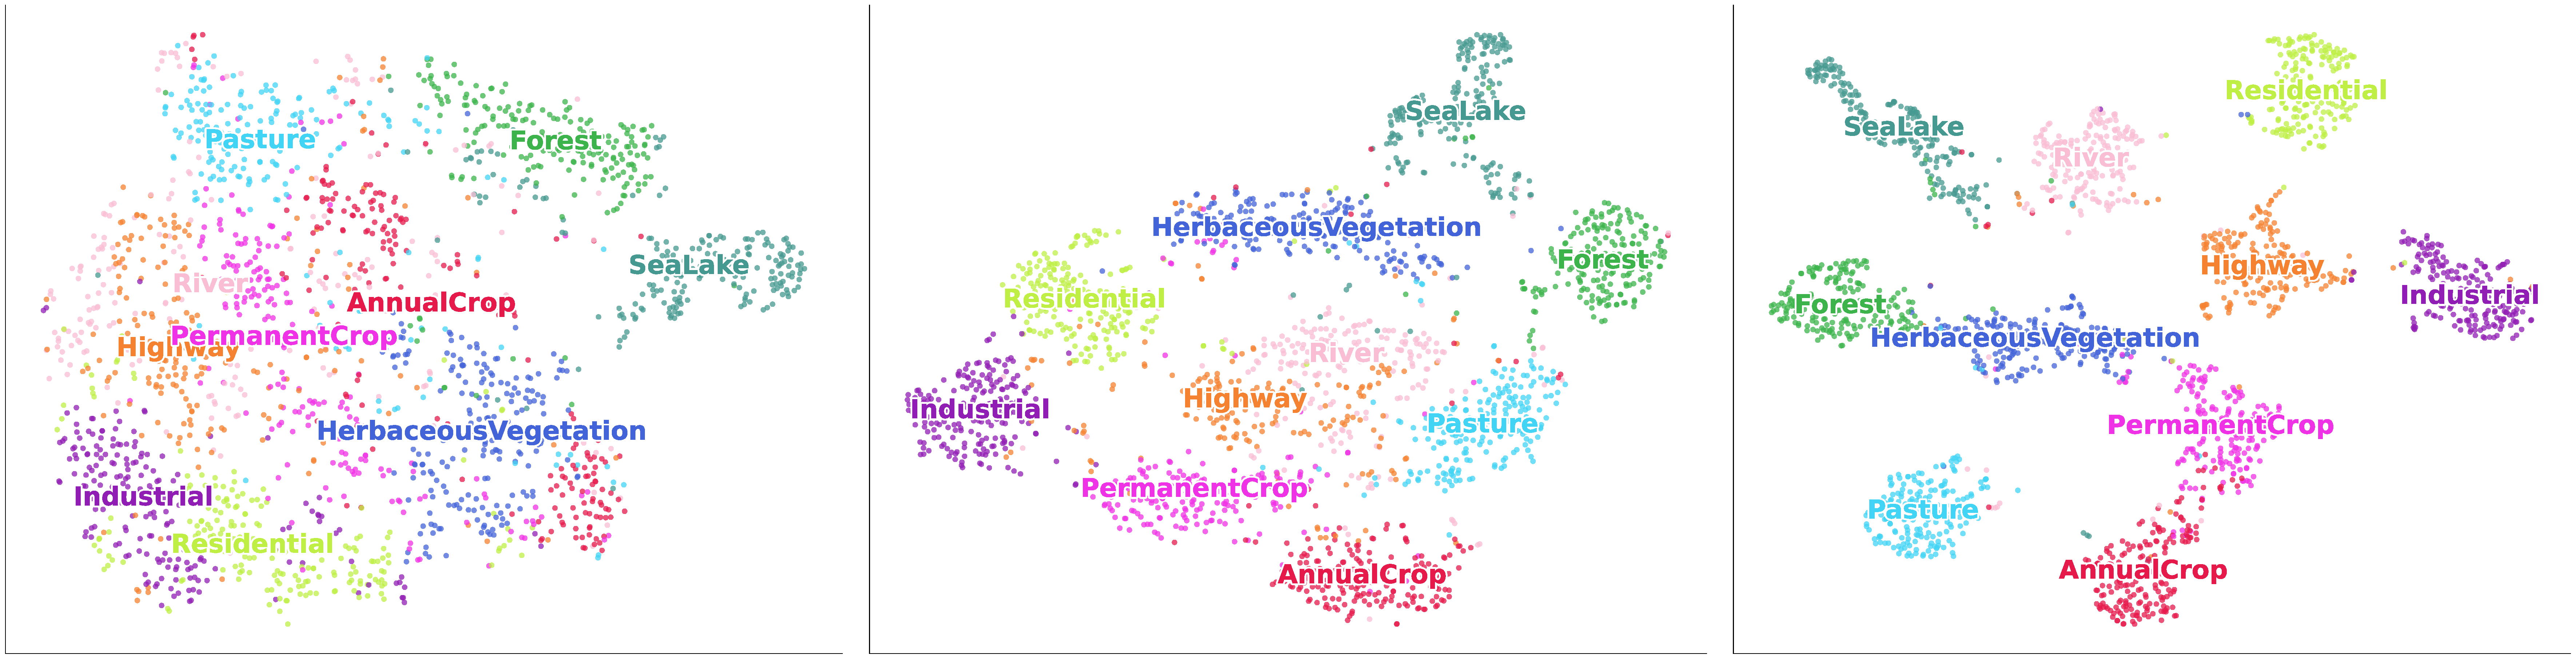
\includegraphics[width=\columnwidth]{figures/tsne_comparison_eurosat.pdf}

\ \\

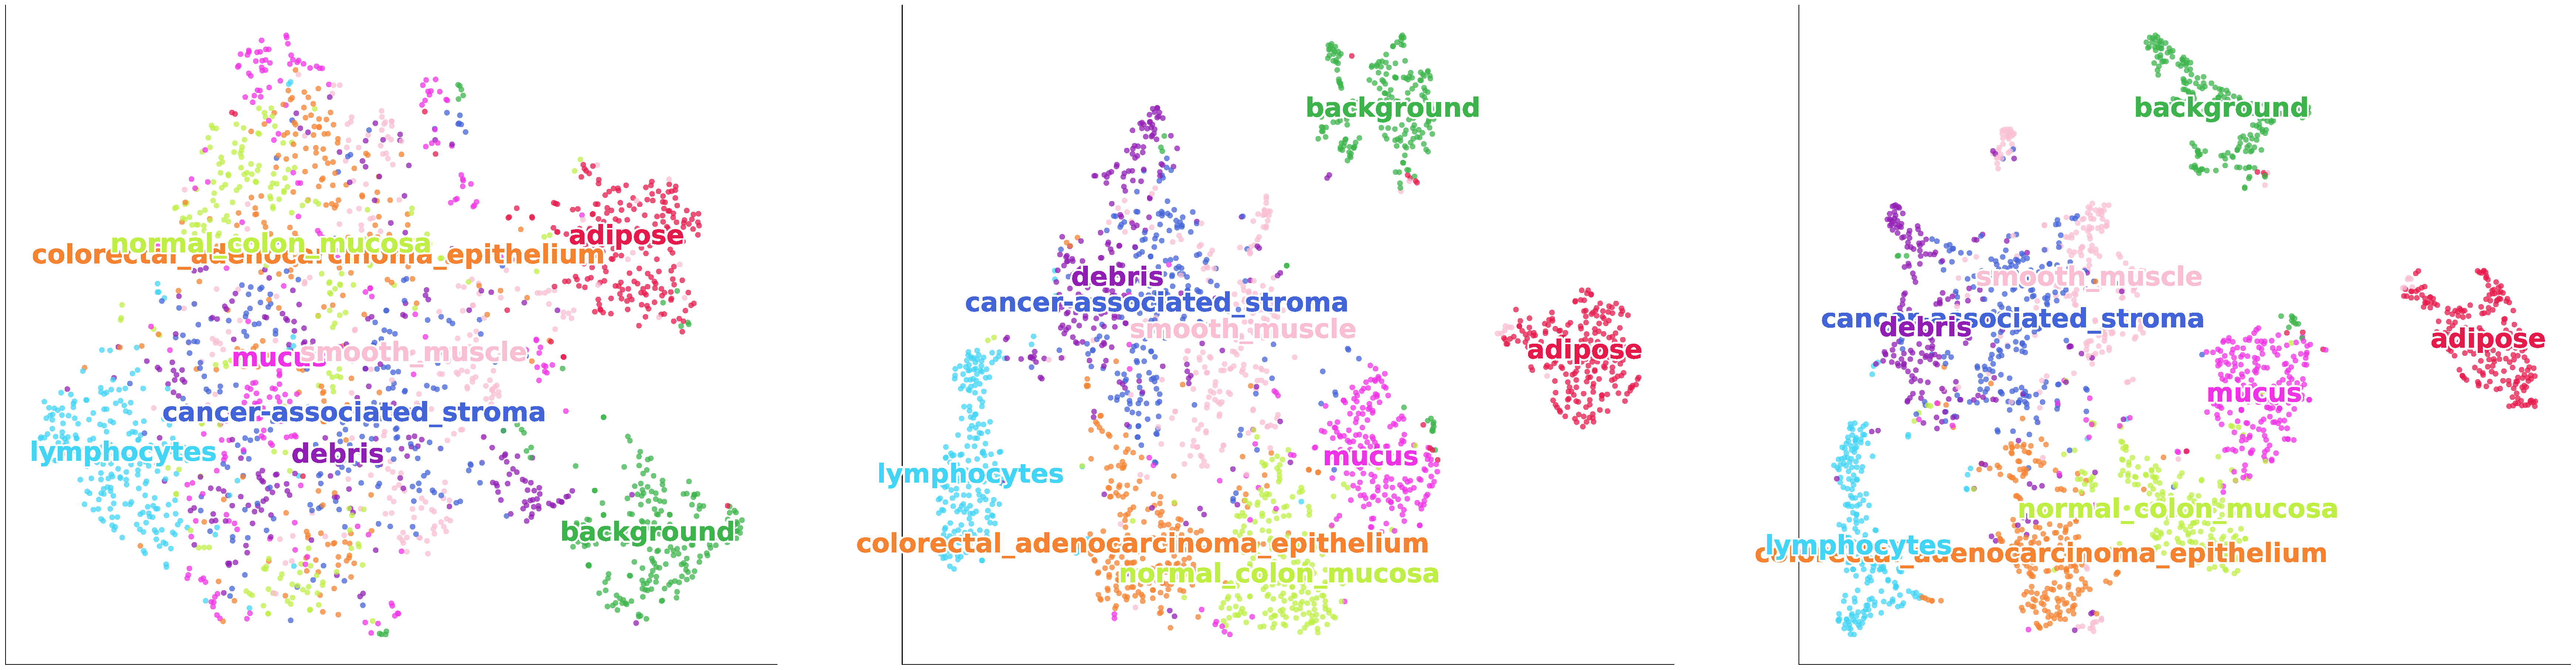
\includegraphics[width=\columnwidth]{figures/tsne_comparison_pathmnist.pdf}

%\vspace{0.9em}
%\vspace{0.4em}
\caption{\textbf{t-SNE visualisations of SAE latent activations: G-SAE vs FT-SAE for datasets EUROSAT(top) and PathMNIST(Bottom)}
Each panel shows patch-level SAE activations projected to 2D via t-SNE, coloured by class label.
Domain-matched SAEs produce more compact, class-separable clusters, especially on far-domain benchmarks,
consistent with the lower label entropy and higher downstream accuracy in
Table~\ref{fig:label_entropy} and Table~\ref{tab:main_accuracy_abs}.}
\label{fig:tsne}
\vspace{-10pt}
\end{figure}


\textbf{Finding 1 — FT-SAES are sparser.}
Applying the generic SAE to LoRA-adapted features forces the model to activate
many neurons just to reconstruct the shifted activations.



Retraining eliminates this waste:
for CLIP, the near-domain average $L_0$ drops from $47$ to $32$ ($-32\%$);
for EuroSAT it drops from $125$ to $15$ ($-88\%$).
Figure~\ref{fig:l0_sparsity} shows this pattern across all four backbones.




The notable exception is DINO on PathMNIST where $L_0$ \emph{increases}
($9{,}185 \to 9{,}676$) and CosSim collapses to $0.013$:
DINOv2's self-supervised features are not sparse-decomposable on medical imagery
(see Sec.~\ref{sec:obs:dino} for discussion).

\textbf{Finding 2 — Dead-neuron fraction mostly decreases, with one instructive exception.}
FT-SAE reduce dead neurons by $31\%$ on average in near-domain settings
(Fig.~\ref{fig:dead_fraction}).
The exception is EuroSAT, where the dead fraction \emph{rises} from $0.16$ to $0.81$.
Combined with an $L_0$ drop from $125$ to $15$ and a CosSim gain of $+0.105$,
this suggests that the FT-SAE creates a \emph{hyper-specialised} dictionary:
a small number of satellite-specific neurons carry all the signal,
while the rest remain dormant.
In this setting, a high dead-neuron fraction is better interpreted alongside sparsity and
reconstruction fidelity, rather than as an isolated failure signal.

\textbf{Finding 3 — Reconstruction fidelity improves except under one dissociation.}
FT-SAES improve average CosSim by $+0.022$ across all backbones and datasets
(Fig.~\ref{fig:paired_cossim}).
DTD stands out: generic SAE NMSE is $0.762$; FT-SAEs NMSE is $0.415$,
a 46\% reduction, indicating that texture domains are especially poorly served
by an ImageNet-pretrained dictionary.
One notable inversion is CLIP PathMNIST where CosSim \emph{drops}
($0.882 \to 0.730$) with the FT-SAE, yet accuracy rises as discussed in \ref{sec:exp:h1}

This dissociation suggests that cosine similarity with the \emph{base} feature space
is not a reliable proxy for downstream utility under large domain shift ---
the FT-SAE discovers new feature directions that are orthogonal to the
pretraining ones yet more useful for the task.
We return to this in Sec.~\ref{sec:obs:cossim}.


Each panel shows patch-level SAE activations projected to 2D via t-SNE, coloured by class label.
Domain-matched SAEs produce more compact, class-separable clusters, especially on far-domain benchmarks
(EuroSAT, PathMNIST, ChestMNIST), consistent with the lower label entropy and higher downstream accuracy in
Table~\ref{fig:label_entropy} and Table~\ref{tab:main_accuracy_abs}.
UCF-101 and DTD show smaller but consistent improvements.
\label{fig:tsne}

\vspace{-4pt}
\paragraph{H3: Standard monosemanticity metrics overestimate interpretability under shift.}
\label{sec:exp:h3}

\vspace{-4pt}
\subparagraph{Domain-Aware Monosemanticity Score.}
A generic SAE can appear spuriously monosemantic on a shifted distribution because
unfamiliar inputs may be consistently mapped to a small set of generic
``catch-all'' features. The standard monosemanticity score $\mathrm{MS}_h$
can therefore be inflated: a latent may fire on a semantically coherent subset,
or even broadly across the target domain, without carrying useful
class-discriminative information. This failure is especially likely when the
target-domain data are poorly represented by the SAE dictionary.
\vspace{-4pt}
\begin{equation}
\label{eq:dams}
\mathrm{DAMS}
=
\mathrm{EC}
\left[
\alpha\,\mathrm{CSS}_{\mathrm{norm}}
+
(1-\alpha)\,\mathrm{FSS}
\right],
\qquad
\mathrm{CSS}_{\mathrm{norm}}
=
\frac{\mathrm{CSS}_{\mathrm{raw}}}
{\mathrm{CSS}_{\mathrm{raw}}+\kappa}.
\end{equation}



Here, $\mathrm{EC}$ measures effective representation coverage and penalises
poorly fitting SAEs whose activations are broad or uninformative.
$\mathrm{CSS}_{\mathrm{raw}}$ measures class-distribution separability in SAE
activation space, while $\mathrm{FSS}$ measures feature-level specificity within
the target label distribution. The parameter $\alpha\in[0,1]$ controls the
trade-off between distribution-level separability and feature-level specificity,
and $\kappa>0$ controls the saturation of the normalized CSS term.

Thus, DAMS is high only when an SAE both preserves useful target-domain
representation structure and produces sparse features that are class-specific.
A generic SAE on a far-domain benchmark may obtain high $\mathrm{MS}_h$ due to
broad, non-discriminative firing, but it should obtain lower DAMS because such
features have weak effective coverage and poor class separability.



\begin{table*}[bp]
\centering
\begin{minipage}[t]{0.45\textwidth}
\centering
\caption{\textbf{MS vs.\ DAMS across datasets (ordered by MMD).}
\textbf{MS}: activation-weighted semantic coherence~\cite{pach2025monosemantic}.
\textbf{DAMS}: Domain-Aware Monosemanticity Score (ours).
}
\label{tab:combined_ms_dams}
\vspace{4pt}
\resizebox{\textwidth}{!}{%
\setlength{\tabcolsep}{3.5pt}
\renewcommand{\arraystretch}{0.95}
\begin{tabular}{l cc ccc}
\toprule
 & \multicolumn{2}{c}{\textbf{MS}} & \multicolumn{3}{c}{\textbf{DAMS}} \\
\cmidrule(lr){2-3}\cmidrule(lr){4-6}
\textbf{Dataset} & G-SAE & FT-SAE & G-SAE & FT-SAE & $\Delta$ \\
\midrule
Caltech101 & 0.657 & \textcolor{red}{0.610} & 0.620 & \textcolor{red}{0.563} & \textcolor{red}{--0.057} \\
DTD        & 0.520 & 0.540                   & 0.300 & {0.585}         & +0.285 \\
UCF101     & 0.687 & 0.690                   & 0.678 & {0.818}         & +0.140 \\
FGVC       & 0.743 & 0.760                   & 0.280 & {0.500}         & +0.500 \\
EuroSAT    & 0.750 & 0.756                   & 0.676 & \textcolor{red}{0.629} & \textcolor{red}{--0.047} \\
PathMNIST  & 0.840 & 0.880                   & 0.682 & {0.980}         & +0.298 \\
\bottomrule
\end{tabular}%
}
\end{minipage}%
\hfill
\begin{minipage}[t]{0.52\textwidth}
\centering
\caption{\textbf{Ablation: SAE expansion factor and training set.}
G-SAE is trained either on ImageNet or on CC3M %$_k$: Generic SAE (ImageNet, $\times k$).
%FT-SAE: LoRASAE ($\times 64$).
\textbf{Bold}: best SAE result.}
\label{tab:expansion_ablation}
\vspace{4pt}
\resizebox{\textwidth}{!}{%
\setlength{\tabcolsep}{2.5pt}
\renewcommand{\arraystretch}{0.95}
\begin{tabular}{lc ccccccc}
\toprule
\rotatebox{0}{\textbf{Method}}
  & \rotatebox{90}{\textbf{Exp.}}
  & \rotatebox{90}{Caltech101}
  & \rotatebox{90}{Oxford Pets}
  & \rotatebox{90}{FGVC}
  & \rotatebox{90}{DTD}
  & \rotatebox{90}{UCF101}
  & \rotatebox{90}{EuroSAT}
  & \rotatebox{90}{PathMNIST} \\
\midrule
LoRA-FT          & ---         & 96.1 & 93.5 & 46.4 & 72.0 & 77.6 & 90.8 & 90.5 \\
\cmidrule(l){1-9}
G-SAE (IN)       & $\times32$  & 89.8 & 85.4 & 33.2 & 62.1 & 66.8 & 81.3 & 78.5 \\
G-SAE (IN)       & $\times64$  & 92.4 & 88.6 & 37.1 & 65.8 & 70.4 & 85.0 & 82.9 \\
G-SAE (IN)       & $\times128$ & 93.1 & 89.5 & 38.4 & 66.9 & 71.6 & 86.2 & 83.8 \\
\cmidrule(l){1-9}
G-SAE (CC3M)     & $\times64$  & 47.8 & 28.3 &  5.8 & 35.7 & 43.3 & 49.8 & 31.0 \\
\cmidrule(l){1-9}
FT-SAE           & $\times64$  & \bf 95.7 & \bf 92.4 & \bf 44.5 & \bf 71.8 & \bf 76.2 & \bf 90.7 & \bf 88.7 \\
\bottomrule
\end{tabular}%
}
\end{minipage}
\end{table*}

\vspace{-4pt}
\paragraph{H4: The interpretability gap scales with domain shift.}
\label{sec:exp:h4}

\textbf{Claim.}
The gap between generic-SAE and FT-SAE quality (on all H1--H3 metrics) grows
monotonically with the MMD distance between the pretraining and target distributions,
providing a practical deployment criterion: the further the target domain,
the more necessary it is to retrain the SAE.





H4 is important because it is a prediction about structure, not just a post-hoc explanation
of individual failures. The dictionary-mismatch hypothesis predicts that degradation should
increase with domain distance rather than appear as an arbitrary collection of dataset-specific
effects. This prediction would be weakened if near-domain benchmarks showed large degradation
while far-domain benchmarks showed



little or none.
Table~\ref{tab:main_accuracy_abs} and Fig.~\ref{fig:l0_sparsity} already show this ordering
holds across all 15 benchmarks; the line plot in Fig.~\ref{fig:gap_vs_distance} makes
the monotone relationship explicit.

The practical implication is direct: given a new target domain, a researcher can compute
its MMD distance from ImageNet and use \ref{tab:combined_ms_dams} as a first estimate of whether generic-SAE degradation is likely to justify retraining before running the full comparison.